\documentclass[titlepage,a4paper,oneside,onecolumn,12pt]{article}

\usepackage[top=3cm, bottom=2cm, left=3cm, right=2cm]{geometry}

\usepackage[utf8]{inputenc}
\usepackage{pgfplotstable}
\usepackage{pgfplots}
\usepackage[brazil]{babel}
\usepackage[T1]{fontenc}
\usepackage{amsmath}
\usepackage{amssymb}
\usepackage{dsfont}
\usepackage[section]{placeins}
\usepackage{algorithm}
\usepackage{algpseudocode}
\usepackage[justification=centering]{caption}
\usepackage{multirow}
\usepackage{mathtools}
\usepackage{fancyhdr}
\usepackage{relsize}


\setlength{\headheight}{15.1pt} 

\fancypagestyle{plain}{\fancyfoot[C]{}\fancyhead[R]{\thepage}}
\pagestyle{plain}

\pgfplotsset{compat=1.9}
\usepgfplotslibrary{patchplots}
\usepgfplotslibrary{fillbetween}

\makeatletter
\renewcommand*{\ALG@name}{Algoritmo}
\makeatother
\algrenewcommand\Return{\State \algorithmicreturn{} }%
\renewcommand{\floatpagefraction}{.9}%



\title{Estruturas de Dados Probabilísticas}
\author{Juan Lopes}

%\includeonly{01_intro}
\includeonly{02_concepts,07_graphs}
%\includeonly{03_bloom}
%\includeonly{04_countmin}
%\includeonly{05_minhash,06_hyperloglog}
%\includeonly{06_hyperloglog}
%\includeonly{07_graphs}

\begin{document}

\maketitle

\linespread{1}\selectfont
\tableofcontents

\linespread{1.5}\selectfont
%~~~~~~~~~~~~~~~~~~~~~~~~~~~~~~~~~~~~~~~~~~~~~~~~~~~~~~~~~~~~~~~~~~~~~~~
\section{Introdução}
%~~~~~~~~~~~~~~~~~~~~~~~~~~~~~~~~~~~~~~~~~~~~~~~~~~~~~~~~~~~~~~~~~~~~~~~

A emergência de sistemas que lidam com múltiplos terabytes de dados exigiu que fossem elaboradas novas técnicas para armazenar e processar esses dados. As limitações de tempo, memória e armazenamento, características comuns ao processamento de dados massivos, guiaram a criação de algoritmos e estruturas de dados que levam em conta tais limitações.

Em diversos domínios, armazenar os dados para processá-los posteriormente pode ser inviável. Isto pode ser justificado pelo alto custo de operações em disco ou mesmo pela perda da habilidade de responder rapidamente às mudanças nos dados.

Neste modelo, é preciso deixar de observar os dados como entidades persistentes, mas entendê-los como fluxos, sobre os quais são derivadas análises imediatas \cite{babcock2002models}. Tais fluxos são contínuos, heterogêneos, mutáveis e frequentemente efêmeros. Dado o volume e a natureza virtualmente infinita desses fluxos, é desejável que os algoritmos e estruturas de dados que os processem sejam capazes de computar resultados de forma contínua e em apenas uma passagem, utilizando o mínimo possível de recursos \cite{alon1996space}.

Alguns problemas podem ter algoritmos trivialmente adaptados para funcionar neste modelo de processamento, como o cálculo da média. Outros, entretanto, podem não ser tão adequados. Um exemplo é o problema de calcular a mediana (ou qualquer quantil) em um fluxo de números inteiros, pois o mesmo requer mais de uma passagem pelos dados ou que eles sejam armazenados para computar o resultado. Em \cite{munro1980selection} mostra-se que calcular quantis em uma série com N valores em $p$ passagens pelos dados requer $\Omega(N^{\frac{1}{p}})$ espaço.

Neste trabalho, abordaremos estruturas de dados conhecidas como estruturas de sinopse (\emph{synopsis}) ou esboço (\emph{sketch}) \cite{gibbons1999synopsis}. Neste trabalho iremos nos referir a elas apenas como estruturas de dados probabilísticas. A principal característica destas é utilizar uma quantidade limitada de recursos. Em especial:

\begin{itemize}
  \item podem residir na memória principal, evitando operações de E/S;
  \item permitem atualização incremental;
  \item consomem menos recursos que os dados originais consumiriam, se fossem armazenados;
  \item podem ser facilmente transmitidas ou armazenadas;
  \item servem como substitutos de baixo custo dos dados originais, viabilizando alguns tipos de consultas.
\end{itemize}

Frequentemente, estruturas de sinopse são pequenas demais para representar fielmente os dados originais e permitir uma resposta exata às consultas. Estas estruturas de dados aproximam a resposta com um fator de erro relativo à quantidade de recursos destinados ao processamento.

Em especial, este trabalho foca nas estruturas que se aproveitam da codificação em \emph{hash} dos elementos de um conjunto ou multiconjunto para responder consultas específicas.

O trabalho está organizado da seguinte maneira: na Seção~\ref{sec:concepts}, introduziremos os conceitos básicos necessários para compreender as estruturas que serão apresentadas nas seções seguintes.

Na Seção~\ref{sec:bloom}, abordamos o filtro de Bloom \cite{bloom1970space}, uma estrutura de dados que responde consultas aproximadas de pertinência de elementos em um conjunto utilizando menos memória do que o necessário para armazenar o conjunto inteiro. É característica dos filtros de Bloom que as respostas negativas sejam exatas, enquanto as respostas positivas sejam aproximadas.

Na Seção~\ref{sec:countmin}, consideramos a estrutura probabilística \emph{count-min} \cite{cormode2005improved}, que é análoga aos filtros de Bloom, permitindo estimar não só a pertinência, mas também a frequência de um elemento em um multiconjunto. Analogamente, qualquer frequência estimada pela estrutura é garantidamente maior ou igual à frequência real do elemento no multiconjunto. É também possível empregá-la para estimar quantis em um fluxo de dados. O texto nesta versão ainda está incompleto e será terminado no futuro.

Na Seção~\ref{sec:minhash} introduzimos o \emph{MinHash} \cite{broder1997resemblance}, estrutura que permite estimar a semelhança entre dois conjuntos sem precisar compará-los elemento a elemento.

Na Seção~\ref{sec:hyperloglog}, abordamos a estrutura \emph{HyperLoglog} \cite{flajolet2008hyperloglog}, que responde a cardinalidade aproximada de elementos distintos de um fluxo de dados utilizando memória adicional constante.

Na Seção~\ref{sec:proposed}, discutimos algumas propostas de continuação deste trabalho.
%~~~~~~~~~~~~~~~~~~~~~~~~~~~~~~~~~~~~~~~~~~~~~~~~~~~~~~~~~~~~~~~~~~~~~~~
\section{Conceitos Básicos}\label{sec:concepts}
%~~~~~~~~~~~~~~~~~~~~~~~~~~~~~~~~~~~~~~~~~~~~~~~~~~~~~~~~~~~~~~~~~~~~~~~

A fim facilitar o entendimento dos conceitos explorados nos próximos capítulos, introduzimos aqui os conceitos básicos utilizados ao longo deste trabalho.

Em especial, abordaremos alguns conceitos básicos de probabilidade, explicando desde o conceito de espaço amostral até variáveis aleatórias e estimadores; conceitos essenciais para explicar e demonstrar as propriedades de estruturas de dados probabilísticas. 

Além disso, faremos uma revisão do estado da arte sobre funções \emph{hash} e modelos de fluxo de dados, que serão bastante referenciados ao longo deste trabalho.

\subsection{Introdução à probabilidade}

O assunto estruturas de dados probabilísticas claramente depende muito da teoria e notações da cálculo de probabilidades. Neste trabalho, a fim de facilitar o entendimento, introduzimos o assunto utilizando notação definida em \cite{figueiredo2007randomizados}.

\subsubsection{Espaço probabilístico}

Define-se o \emph{espaço probabilístico} como formado por dois componentes: um \emph{espaço amostral} $\Omega = \{r_1, r_2, \cdots\}$, que representa os possíveis resultados de um experimento aleatório, e uma \emph{função de probabilidade} $\Pr$, que define a probabilidade com que qualquer \emph{evento} $A \subseteq \Omega$ ocorre em experimentos aleatórios. Esta função precisa respeitar as seguintes propriedades:

\begin{enumerate}
  \item Para todo evento $A \subseteq \Omega$, $0 \leq \Pr[A] \leq 1$.
  \item $\Pr[\Omega] = 1$.
  \item Para eventos $A_1, A_2, ..., A_n$ disjuntos, $\Pr[\bigcup_i A_i] = \sum_i \Pr[A_i]$.
\end{enumerate}

No caso de eventos $A_1, A_2, ..., A_n$ arbitrários (isto é, não necessariamente disjuntos), vale o \emph{princípio da inclusão-exclusão}:
\begin{alignat*}{2}
    \Pr\left[ \bigcup_i A_i \right] = & \sum_i \Pr[A_i] \\
                                  & - \sum_{i<j} \Pr[A_i \cap A_j] \\
                                  & + \sum_{i<j<k} \Pr[A_i \cap A_j \cap A_k] \\
                                  & - \cdots \\
                                  & + (-1)^{l+1} \sum_{i_1 < i_2 < \cdots < i_l} \Pr \left[ \bigcap_{r=1}^{l} A_{i_r} \right] \\
                                  & + \cdots
\end{alignat*}
e em especial
\[
    \Pr[A_1 \cup A_2] = \Pr[A_1] + \Pr[A_2] - \Pr[A_1 \cap A_2]
\]

Como exemplo destes conceitos, podemos analisar as probabilidades envolvidas no lançamento de um dado de seis lados. Definimos $\Omega = \{1, 2, 3, 4, 5, 6\}$, representando todos os possíveis resultados deste experimento. 

Sabemos que a probabilidade de qualquer resultado $E_i = \{r_i\}, r_i \in \Omega$ é igual, isto é $\Pr[E_i] = {^{1}/_{6}}$. Podemos calcular que a probabilidade de um lançamento resultar em 2 ou 5 é dada pela probabilidade da união entre os dois eventos que, para conjuntos disjuntos, é igual a: $\Pr[\{2, 5\}] = \Pr[\{2\}] + \Pr[\{5\}] = {^2/_6} = {^1/_3}$.

Entretanto, para calcular a probabilidade do resultado ser um número divisível por dois (evento \textsc{Div2}) ou por três (evento \textsc{Div3}) podemos utilizar o princípio da inclusão-exclusão. Assim 
\[
\Pr[\textsc{Div2} \cup \textsc{Div3}] = \Pr[\textsc{Div2}] + \Pr[\textsc{Div3}] - \Pr[\textsc{Div2} \cap \textsc{Div3}]
\]
ou seja,
\begin{alignat*}{2}
\Pr[\{2,4,6\} \cup \{3,6\}] &= \Pr[\{2,4,6\}] + \Pr[\{3,6\}] - \Pr[\{6\}] \\
                            &= {^3/_6} + {^2/_6} - {^1/_6} \\
                            &= {^4/_6}
\end{alignat*}

\subsubsection{Variáveis aleatórias}

Uma \emph{variável aleatória} $X$ é uma função que mapeia o espaço amostral em um outro conjunto. Neste trabalho apenas lidaremos com variáveis aleatórias reais, na forma $X : \Omega \to \mathbb{R}$. 

A função \emph{densidade de probabilidade} de uma variável aleatória real é definida como $p_X(x) : \mathbb{R} \to [0, 1]$. $p_X(x) = \Pr[X = x]$, que é outra forma de escrever $\Pr[\{r \in \Omega \mid X(r) = x\}]$, ou seja, a probabilidade do resultado $r$ de um experimento aleatório seja tal que $X(r) = x$.

O valor esperado (ou esperança) de uma variável aleatória consiste na média de todos os possíveis valores que ela pode assumir, ponderada pela probabilidade que cada valor tem de ser assumido. Isto é,
\[
    \text{E}[X] = \sum_{x \in \mathbb{R}} x p_X(x).
\]

Por exemplo, considere o resultado do lançamento de dois dados de seis lados. Podemos definir a variável $X$ como a soma dos valores obtidos nos dados. Assim, temos por exemplo que $p_X(3) = {^2/_{36}}$, pois apenas dois resultados possíveis neste experimento resultam na soma 3 ($1+2$ e $2+1$). Por outro lado, $p_X(7) = {^6/_{36}}$, pois seis resultados possíveis no espaço amostral somam 7 ($1+6$, $2+5$, etc.). Assim, o valor esperado para a variável $X$ é:
\begin{align*}
    \text{E}[X] &= 2 \cdot p_X(2) + 3 \cdot p_X(3) + ... + 12 \cdot p_X(12) \\
          &= 2 \cdot {^1/_{36}} + 3 \cdot {^2/_{36}} + ... + 12 \cdot {^1/_{36}} \\
          &= 7
\end{align*}

A \emph{linearidade da esperança} é a propriedade que diz que, para variáveis aleatórias $X_1, X_2, \cdots, X_n$ e uma função linear $h$, vale:
\[
    \text{E}[h(X_1, X_2, \cdots, X_n)] = h(\text{E}[X_1], \text{E}[X_2], \cdots, \text{E}[X_n])
\]

Ainda utilizando o exemplo do lançamento de dois dados, uma outra forma de calcular o valor esperado seria fazê-lo para apenas um dado e dobrar o resultado. Considere as variáveis aleatórias $Y_1$ e $Y_2$ como os valores resultantes do lançamento de cada um dos dados, tal que $X = Y_1 + Y_2$. Assim, pela linearidade da esperança, $\text{E}[X] = \text{E}[Y_1 + Y_2] = \text{E}[Y_1] + \text{E}[Y_2]$. 

O valor esperado para $Y_i$ é mais fácil de calcular, sendo apenas a média simples entre todos os resultados possíveis no lançamento de um dado:
\[
    \text{E}[Y_i] = \frac{1+2+3+4+5+6}{6} = \frac{21}{6} = \frac{7}{2}
\]
logo
\[
    \text{E}[X] = \text{E}[Y_1] + \text{E}[Y_2]  = \frac{7}{2} + \frac{7}{2} = 7
\]

Uma propriedade importante de variáveis aleatórias é sua variância, que pode ser definda da seguinte forma:
\[
    \text{Var}[X] = \text{E}[(X - \text{E}[X])^2] = \text{E}[X^2] - (\text{E}[X])^2
\]

Dadas variáveis aleatórias independentes $X_1, X_2, \cdots, X_n$, todas com a mesma variância $\sigma^2$, a \emph{fórmula de Bienaymé} reza sobre a variância da média $\bar{X}$ dessas variáveis:
\[
    \text{Var}[\bar{X}] = \text{Var}\left[ \frac{1}{n} \sum_{i=1}^{n} X_i \right] = \frac{1}{n^2} \sum_{i=1}^{n} \text{Var}[X_i]  = \frac{\sigma^2}{n}
\]

Isto significa, na prática, que a média entre $n$ variáveis independentes diminui a variância por um fator de $n$. Este resultado é útil para estruturas de dados probabilísticas, pois permite diminuir o erro compondo estimadores independentes.

Algumas variáveis aleatórias são muito comumente vistas na teoria e possuem muitas propriedades já estudadas. Para este trabalho iremos focar na variável de \emph{Bernoulli} e na variável \emph{binomial}, sendo a primeira apenas um caso especial da segunda.

A variável de Bernoulli pode assumir apenas dois valores: 0 ou 1. Ela representa o resultado de um experimento onde o valor 0 representa um "fracasso" e o valor 1 um "sucesso". Seja $p$ a probabilidade de sucesso, temos que
\[
    p_X(x) = \begin{cases}
        1 - p  & \text{se } x = 0 \\
        p      & \text{se } x = 1 \\
        0      & \text{para demais valores de } x \\
        
    \end{cases}
\]

É fácil demonstrar que para uma variável de Bernoulli $X$, $\text{E}[X] = p$ e $\text{Var}[X] = p (1-p)$.

A variável binomial representa o total de sucessos em uma série de $n$ experimentos e pode ser vista como o somatório de $n$ variáveis de Bernoulli com uma mesma probabilidade $p$.

Denota-se $B(n, p)$ a variável binomial que representa o total de sucessos de $n$ experimentos com probabilidade $p$. A densidade de probabilidade desta variável é
\[
    p_{B(n,p)} = \begin{cases}
        {\binom{n}{x}} p^x(1-p)^{n-x}    & \text{para } 0 \leq x \leq n \\
        0                               & \text{para demais valores de x} \\
    \end{cases}
\]

O valor esperado da variável binomial pode ser inferido pela linearidade da esperança de cada variável de Bernoulli que a compõem, ou seja $E[B(n, p)] = np$. 

A partir da definição $\text{E}[X^2] = n (n-1) p^2 + np$, podemos calcular a variância da variável binomial: $\text{Var}[X] = np(1-p)$.

Perceba que a variável de Bernoulli é apenas um caso especial de uma variável binomial, $B(1, p)$.

\subsubsection{Desigualdades probabilísticas}

Embora o valor esperado de uma variável aleatória nos forneça valiosa informação sobre como uma variável se comporta na média de vários experimentos, ele não nos diz muito sobre a distribuição dos valores que a variável pode assumir.

Ao utilizar estruturas de dados probabilísticas, por exemplo, calculamos o valor de variáveis aleatórias cujo valor esperado é igual ao que se deseja estimar. Entretanto, para ter alguma utilidade prática, é preciso poder prever a probabilidade de erro.

A seguir apresentaremos algumas desigualdades que permitem definir um limite superior na probabilidade da variável aleatória assumir certos intervalos de valores.

A \emph{desigualdade de Markov}, por exemplo, diz que para variáveis $X$ que somente assumem valores não-negativos,
\[
    \Pr[X \geq a] \leq \frac{\text{E}[X]}{a} \text{, para todo } a > 0
\].

Se a variância da variável for conhecida, um limite mais forte pode ser estabelecido, através da \emph{desigualdade de Chebyshev}:
\[
    \Pr[|X - \text{E}[X]| \geq a] \leq \frac{\text{Var}[X]}{a^2} \text{, para todo } a > 0
\]

É possível reescrever esta desigualdade definindo o desvio padrão $\sigma = \sqrt{\text{Var}[X]}$. Assumindo $a = k\sigma$,
\[
    \Pr[|X - \text{E}[X]| \geq k\sigma] \leq \frac{1}{k^2} \text{, para todo } k > 1
\]

Este limite mostra, de forma intuitiva, como as probabilidades de cada um dos valores de $X$ se comportam conforme eles se afastam de $\text{E}[X]$.

Sem mais informações sobre a variável não é possível definir limites gerais mais fortes para sua distribuição. Entretanto, para alguns tipos de variáveis específicas é possível utilizar a \emph{desigualdade de Chernoff} para encontrar limites específicos desta distribuição. Existem diversas variantes desta desigualdade, cada uma específica para um tipo de variável aleatória. Em especial, abordaremos aqui o uso desta desigualdade para variáveis de Bernoulli.

Considere uma variável $X = \sum_{i=1}^n X_i$, onde todo $X_i$ é uma variável de Bernoulli independente com probabilidade $p_i$. Seja também $\mu = \text{E}[X] = \sum_{i=1}^n p_i$. Então, dois limites se aplicam:

\begin{itemize}
  \item \textbf{Limite superior:} $\Pr[X \geq (1 + \delta)\mu] \leq e^{-\frac{\delta^2}{2+\delta}\mu}$ para todo $\delta > 0$;
  \item \textbf{Limite inferior:} $\Pr[X \leq (1 - \delta)\mu] \leq e^{-\mu\delta^2/2}$ para todo $0 < \delta < 1$;
\end{itemize}

Uma versão simplificada que combina combina os dois limites é definida por
\[
    \Pr[|X - \mu| \geq \delta\mu] \geq 2e^{-\mu\delta^2/3}\text{ para todo } 0 < \delta < 1.
\]

\subsubsection{Estimadores}

Um estimador é uma regra que permite estimar um certo parâmetro $\theta$ de uma variável aleatória $X$ a partir de observações sobre a mesma. São funções denotadas $\hat{\theta} : E \to \Theta$, onde $E$ é o contra-domínio da variável $X$ e $\Theta$ é chamado de espaço paramétrico.

Estimadores também são variáveis aleatórias por si só, portanto possuem média, variância, desvio padrão etc.

O viés de um estimador é a diferença entre seu valor esperado e o parâmetro que ele almeja estimar, ou seja, $\text{B}(\hat{\theta}) = \text{E}[\hat{\theta}] - \theta$. Um estimador é considerado \emph{não-enviesado} se e somente se $\text{B}(\hat{\theta}) = 0$.

A variância de um estimador é um parâmetro importante para analisar seu erro padrão. A variância, assim como em uma variável aleatória, mede o quanto cada observação se afasta de seu valor valor esperado e é definida como:
\[
    \text{Var}[\hat{\theta}] = \text{E}[(\hat{\theta} - \text{E}[\hat{\theta}])^2] = \text{E}[\hat{\theta}^2] - (\text{E}[\hat{\theta}])^2
\]

Consequentemente, o erro padrão de um estimador é definido como $\sigma_{\hat{\theta}} = \sqrt{\text{Var}[\hat{\theta}}]$.

O erro médio quadrático (EMQ) de um estimador combina variância e viés em um único conceito. Em vez de comparar a diferença entre cada observação e o valor esperado do estimador, compara-se com o valor real do parâmetro. Isto é $\text{EMQ}[\hat{\theta}] = \text{E}[(\hat{\theta} - \theta)^2]$. Em um estimador não-enviesado, o EMQ é igual à variância.

\subsection{Funções \emph{hash}}

Todas as estruturas descritas neste trabalho são baseadas em funções \emph{hash} e são, de certa forma, dependentes das propriedades das funções utilizadas. Por isso, apresentamos aqui um breve resumo das características principais esperadas de funções aplicáveis a estruturas de dados probabilísticas.

O objetivo principal das funções \emph{hash} neste contexto é a capacidade de simular certa aleatoriedade a um conjunto de dados que pode ter um grau de entropia muito baixo. Como Knuth diz em \cite{knuth1998art}, é impossível definir uma função que cria dados aleatórios a partir de dados não aleatórios, mas na prática é possível criar uma imitação boa o suficiente.

\subsubsection{Tabelas \emph{hash}}

A aplicação mais direta de funções \emph{hash} é a possibilidade de mapear chaves contidas em conjuntos muito grandes a entradas numa tabela com tamanho potencialmente bem menor do que os conjuntos que representam, uma tabela \emph{hash}. Por exemplo, é possível mapear \emph{strings}, um conjunto infinito, para inteiros na tabela, de forma que a complexidade esperada para verificar sua existência seja independente do tamanho da tabela, e sim proporcional ao tamanho da \emph{string}. A Figura~\ref{fig:hashtable} mostra um exemplo deste tipo de tabela.

\begin{figure}[!htbp]
  \centering
  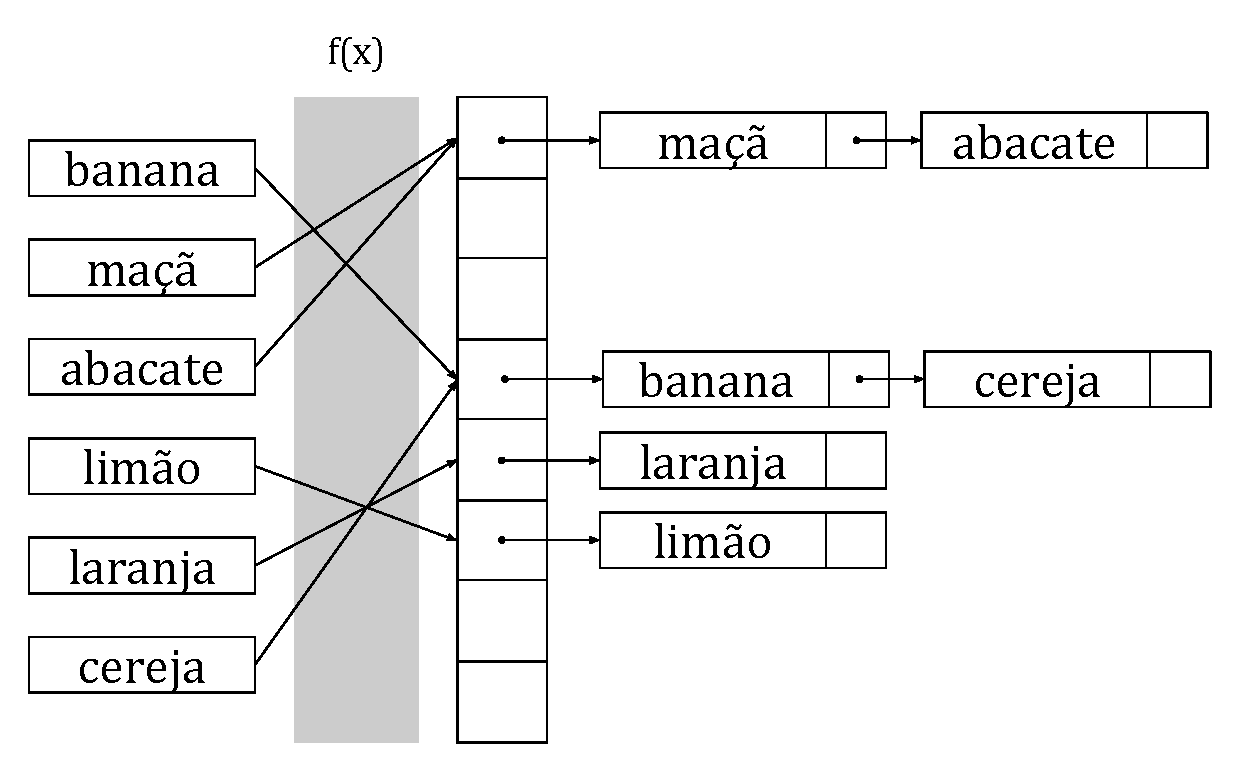
\includegraphics[scale=0.6]{files/hashtable.pdf}
  \caption{Exemplo de tabela \emph{hash}}
  \label{fig:hashtable}
\end{figure}

O exemplo dado assume algumas propriedades da função \emph{hash} escolhida, em especial:
\begin{itemize}
  \item \textbf{A distribuição da imagem é aparentemente uniforme:} isto é, a probabilidade aparente de qualquer um dos valores do contradomínio ser escolhido para representar a entrada é igual. Esta é uma propriedade impossível de alcançar na teoria e sua aplicação prática pode ser amplamente dependente do domínio da função, por exemplo: uma função \emph{hash} que funciona bem para palavras em português pode não funcionar tão bem para palavras em inglês.
  
  \item \textbf{A função tem baixa complexidade (linear, de preferência):} Funções com complexidades maiores podem tornar a inserção e busca na tabela inviáveis.
  
  \item \textbf{A função é determinística:} esta é uma propriedade redundante, se assumirmos a definição usual de \emph{função}, entretanto dado o contexto é importante explicitá-la, visto que uma função \emph{hash} que resulta em valores diferentes (se aplicada várias vezes à mesma entrada) não tem valor para busca em tabelas. Dito isto, os conceitos de funções pseudo-aleatórias e funções \emph{hash} possuem grande interseção teórica.
\end{itemize}

Há outros detalhes teóricos e de implementação de tabelas \emph{hash} que não serão tratados aqui (como a resolução de colisões por exemplo), por não dizerem tanto a respeito de funções \emph{hash} em si, que são o foco desta seção.

\subsubsection{\emph{Hashs} criptográficos}

Não há um conjunto ideal de propriedades de funções \emph{hash} que sirva a todos os propósitos possíveis. As propriedades ideais para uso em uma tabela \emph{hash} não são os mesmos para o uso em aplicações de segurança, por exemplo. Nestas, é usualmente requerido que um usuário malicioso seja (na prática) incapaz de criar chaves que sejam mapeadas para um valor específico do contradomínio da função. Isto é, deseja-se que a tarefa encontrar a função inversa da função \emph{hash} seja computacionalmente inviável.

\subsubsection{\emph{Hashing} universal e \emph{HashDOS}}

\subsubsection{Exemplos de funções \emph{hash}}



\subsection{Modelo de processamento em fluxos de dados}


%~~~~~~~~~~~~~~~~~~~~~~~~~~~~~~~~~~~~~~~~~~~~~~~~~~~~~~~~~~~~~~~~~~~~~~~
\section{Filtro de Bloom}\label{sec:bloom}
%~~~~~~~~~~~~~~~~~~~~~~~~~~~~~~~~~~~~~~~~~~~~~~~~~~~~~~~~~~~~~~~~~~~~~~~

Um filtro de Bloom é uma estrutura de dados probabilística que representa um conjunto e permite verificar a pertinência de elementos com tolerância a falsos positivos \cite{bloom1970space}. É uma representação bastante compacta: são necessários menos de 10 bits por elemento para uma probabilidade 1\% de falsos positivos \cite{bonomi2006improved}. 

Nas Seções \ref{sec:bloom:def} e \ref{sec:bloom:example}, apresentamos a definição da estrutura Filtro de Bloom e mostramos um exemplo compreensivo de seu funcionamento. Na Seção~\ref{sec:bloom:false}, calculamos a probabilidade de falsos positivos inerentes ao algoritmo. Na Seção~\ref{sec:bloom:cardinality}, introduzimos uma técnica para estimar cardinalidade de conjuntos utilizando filtro de Bloom. Na Seção~\ref{sec:bloom:counting}, discutimos em detalhe umas das variantes importantes da estrutura que permite remoção de elementos. Outras variantes são discutidas na Seção~\ref{sec:bloom:variants}. Na Seção~\ref{sec:bloom:apps} apresentamos algumas aplicações de filtros de Bloom. E na Seção~\ref{sec:bloom:experiments} mostramos o resultado de experimentos com filtros de Bloom, que visam avaliar o erro observado em uma implementação real.

\subsection{Definição}\label{sec:bloom:def}

Um filtro de Bloom representa um conjunto $S$ de cardinalidade $n$ utilizando um vetor $B$ de $m$ bits. Inicialmente, $B[i] = 0\ \forall\ i \in [1..m]$. O filtro está associado a $k$ funções \emph{hash} $h_i : S \rightarrow [1..m]\ \forall\ i \in [1..k]$. Assume-se que cada função $h_i$ mapeia elementos de $S$ para o intervalo $[1..m]$ de forma aleatória com uma distribuição uniforme.

Para inserir um elemento, é preciso atribuir 1 para cada posição no filtro mapeada pelas funções $h_i$, como mostra o Algoritmo~\ref{alg:bloominsert}.

\begin{algorithm}
\linespread{1}\selectfont
\caption{Adiciona um elemento a um filtro de Bloom}
\label{alg:bloominsert}
\begin{algorithmic}[1]
\Procedure{Inserir}{$x$}
    \For{$i \gets  1 \textrm{ to } k$}
        \State $B[h_i(x)] \gets 1$
	\EndFor
\EndProcedure
\end{algorithmic}
\end{algorithm}

Analogamente, para verificar se um elemento pertence a um conjunto, é preciso verificar se todos os bits mapeados pelas funções $h_i$ estão ligados, i.e., um elemento $x$ provavelmente pertence ao conjunto $S$ se o Algoritmo~\ref{alg:bloomquery} retorna verdadeiro.

\begin{algorithm}
\linespread{1}\selectfont
\caption{Verifica se um elemento pertence a um filtro de Bloom}
\label{alg:bloomquery}
\begin{algorithmic}[1]
\Function{Verificar}{$x$}
    \State $resultado \gets \textbf{true}$ 
    \For{$i \gets  1 \textrm{ to } k$}
        \State $resultado \gets resultado \land B[h_i(x)] = 1$
	\EndFor
	\Return $resultado$
\EndFunction
\end{algorithmic}
\end{algorithm}

A Figura~\ref{fig:bloom1} mostra um exemplo de filtro de Bloom. Do lado esquerdo, estão representadas as operações de inserção, utilizando duas funções \emph{hash}. Do lado direito, as operações de verificação. Importante notar que a última operação de verificação trata o caso de um falso posivito, pois o elemento não existe de fato no conjunto previamente inserido.

\begin{figure}[!htbp]
  \centering
  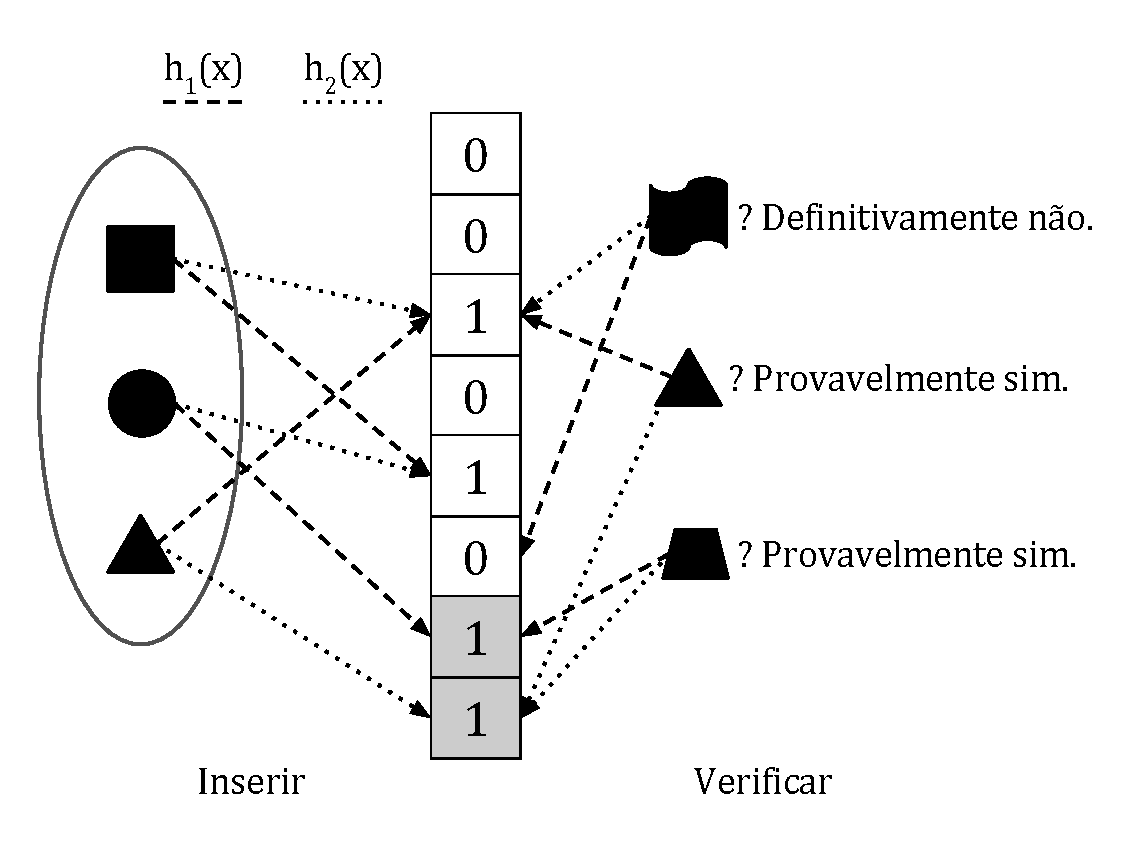
\includegraphics[scale=0.45]{files/bloom1.pdf}
  \caption{Exemplo de filtro de bloom}
  \label{fig:bloom1}
\end{figure}

Em sua forma mais simples, o funcionamento de um filtro de Bloom é similar ao de uma \emph{hash table} tradicional, porém os elementos originais não são armazenados. Em vez disso, apenas um bit é usado para representar a pertinência do \emph{hash} do elemento na tabela. Além disso, múltiplas funções \emph{hash} são utilizadas.

Assim como em \emph{hash tables}, pode haver colisões nos filtros de Bloom. Portanto, falsos positivos são possíveis. Falsos negativos por sua vez não são possíveis Este comportamento é desejado em sistemas que precisam evitar operações custosas (por exemplo, acesso a disco, comunicação de rede, etc.) em casos onde não seja realmente necessário. 

Para diminuir a probabilidade de colisão, é preciso dimensionar o filtro e as funções \emph{hash} baseados no número de elementos esperados. Por exemplo, usando 7 funções e pouco menos de 10 bits por elemento no filtro, é possível garantir uma probabilidade de falsos positivos menor que 1\% \cite{bonomi2006improved}. É possível determinar a quantidade ótima de bits e funções dada uma probabilidade esperada de falsos positivos.

O número de funções \emph{hash} pode posar como um desafio, a princípio. Porém, é resultado conhecido que apenas duas funções independentes são suficientes para gerar qualquer número de funções sem perda das propriedades originais da estrutura \cite{kirsch2006less}.

Em termos de operações suportadas, filtros de Bloom permitem atualização incremental, bem como união entre filtros (que para filtros de mesmo número de bits, consiste em um \emph{OU binário} entre eles). Entretanto, em sua forma mais simples, não suportam remoção de elementos nem interseção entre filtros sem introduzir falsos negativos ou afetar as probabilidades de falsos positivos. Diversas variações e extensões aos filtros de Bloom foram propostas, algumas discutidas nas Seções \ref{sec:bloom:counting} e \ref{sec:bloom:variants}.

\subsection{Exemplo}\label{sec:bloom:example}


\subsection{Probabilidade de falso positivo}\label{sec:bloom:false}

A probabilidade de um falso positivo é determinada pela probabilidade de colisão. Assim, quanto mais bits forem usados no filtro de Bloom, menor a probabilidade de um falso positivo. Para diminuir a probabilidade de colisões é possível também utilizar múltiplas funções \emph{hash} para cada elemento, mas somente até um certo ponto, onde realizar múltiplos hashes por elemento acaba aumentando a probabilidade de colisões.

É possível calcular a probabilidade de um falso positivo. Considere uma tabela $B[1..m]$, após inserir $n$ elementos e usando $k$ funções \emph{hash}. Se $X_i$ é a variável aleatória que fornece o valor de $B[i]$, então:
\[
\Pr[X_i = 0] = \Pr\left[\bigwedge_{x \in X, 1 \leq j \leq k} h_j(x) \neq i \right] = \left( 1 - \frac{1}{m}\right)^{kn}
\]

Seja \textsc{FalsoPositivo} o evento do filtro reportar pertinência para um elemento $x \notin X$. Logo, a probabilidade de haver um falso positivo é a mesma de encontrar $k$ bits 1 aleatoriamente na tabela, ou seja:
\[
\Pr[\textsc{FalsoPositivo}] = \Pr\left[\bigwedge_{1 \leq j \leq k} X_{h_j(x)} = 1 \right] = \left( 1 - \left( 1 - \frac{1}{m}\right)^{kn} \right)^k \approx \left( 1 - \mathrm{e} ^{-kn/m} \right)^k
\]

É fácil ver que a probabilidade de falsos positivos cresce conforme $n$ cresce. Por isso, é preciso dimensionar o filtro de Bloom de acordo com o número de elementos no conjunto. Se definirmos $q = m/n$ (quantidade de bits por elemento, reescrevemos a última probabilidade como:
\[
\Pr[\textsc{FalsoPositivo}] \approx \left( 1 - \mathrm{e} ^{-k/q} \right)^k
\]

A Figura~\ref{fig:probfalso1} mostra como esta probabilidade se comporta para diferentes valores de $k$ e $q$.

\begin{figure}[!htbp]
\centering
\scalebox{0.80}{\begin{tikzpicture}[
        declare function = {
            p(\q,\k) = ((1 - (e^(-\k/\q)))^\k)*100;
        }
    ]
    \begin{axis}[
        view={0}{90}, 
        colorbar, 
        colorbar style={
            ylabel=falsos positivos,
            yticklabels={0, 0.1\%, 1\%, 10\%, 100\%},
        },
        colormap={}{ gray(0cm)=(1); gray(1cm)=(0);},
        xlabel=bits / elemento ($q$),
        ylabel=funções \emph{hash} ($k$),
        xticklabel style={anchor=north west},
        yticklabel style={anchor=south east},
        ytick = { 1, 3, ..., 14},
        xtick = { 1, 3, ..., 14},
        zmode=log,
        log base z=10,
    ]
        \addplot3[surf,domain=1:15,samples=15]{p(x,y)};
    \end{axis}
\end{tikzpicture}}
\caption{Probabilidade de falsos positivos}
\label{fig:probfalso1}
\end{figure}

Bonomi et al. \cite{bonomi2006improved} mostram ainda que a probabilidade é minimizada quando $k = q \ln 2$. Assim, é possível definir a probabilidade mínima de falsos positivos a partir do número de bits por elemento:
\[
\Pr[\textsc{FalsoPositivo}] = (1-e^{\ln(2)}) ^ {q \ln(2)} = ((1/2)^{\ln(2)})^q \approx \left( 0.6185 \right)^q
\]

É possível ver na Figura~\ref{fig:probfalso2} que a probabilidade de falsos positivos cai exponencialmente em relação ao número de bits por elemento no filtro.

\begin{figure}[!htbp]
\centering
\scalebox{0.80}{\begin{tikzpicture}[
        declare function = {
            p(\q) = (0.6185)^(\q);
        }
    ]
	\begin{axis}[
        grid=both,
        xlabel=bits / elemento (q),
		ylabel={Pr[\textsc{FalsosPositivos}]},
        yticklabels={0, 0.001\%, 0.01\%, 0.1\%, 1\%, 10\%, 100\%},
        ymode=log,
        ymax=1,
		xmin=0,
		xmax=25]
	\addplot[mark=*,domain=0:25,samples=26] {p(x)};
	\end{axis}
\end{tikzpicture}}
\caption{Probabilidade mínima de falsos positivos}
\label{fig:probfalso2}
\end{figure}

Desta forma, a escolha do número de bits por elemento torna-se crucial para dimensionar a quantidade de falsos positivos. Esta análise precisa ser feita \emph{a priori}, pois não é possível redimensionar um filtro de Bloom sem modificar suas propriedades estatísticas. 

Existem variações do algoritmo que mitigam este problema. Por exemplo, os \emph{Dynamic Bloom Filters} \cite{guo2010dynamic} colocam um limite superior na probabilidade de falso positivo criando um novo filtro quando o limite é ultrapassado, penalizando as consultas em um fator logaritmico, em relação ao tamnho do conjunto, pois precisam verificar vários filtros. 

Já os \emph{Block-partitioned Bloom Filters} \cite{papapetrou2010cardinality} penalizam tanto a inserção quanto a consulta de forma similar, porém por inserir e verificar os elementos em todos os filtros, mantêm as propriedades algébricas de união entre filtros através de operações booleanas entre seus vetores.

\subsection{Estimativa de cardinalidade}\label{sec:bloom:cardinality}

É possível estimar a cardinalidade do conjunto representado por um filtro de Bloom \cite{whang1990linear,papapetrou2010cardinality}. O princípio é análogo àquele empregado na Seção~\ref{sec:bloom:false} para estimar a probabilidade de falsos positivos. Seja $T$ a variável aleatória que representa o número de bits $1$ após inserir $n$ elementos num filtro $B[1..m]$ e $k$ funções \emph{hash}. Portanto, $T = \sum_{1 \leq i \leq m} X_i = 1$ e a esperança $E[T]$ é uma função $S(n)$ (para $m$ e $k$ fixos) tal que:
\[
E[T] = \sum_{1 \leq i \leq m} E[X_i] = m \times Pr[X_i = 1] = \hat{S}(n) = m \times \left( 1 - \left( 1 - \frac{1}{m}\right)^{kn} \right)
\]

Desta forma, é possível estimar $n$ a partir de $t$:
\[
\hat{n} = \hat{S}^{-1}(t) = \frac{\ln \left( 1 - \frac{t}{m} \right)}{k \times \ln \left( 1 - \frac{1}{m} \right)} \approx \frac{-m}{k} \times \ln \left( 1-\frac{t}{m} \right)
\]

Perceba que esta estimativa é extremamente dependente da quantidade de bits por elemento no filtro. Portanto, dado um certo filtro de Bloom, apenas um intervalo definido de cardinalidades tem um erro entro de um limite aceitável. Papapetrou et al. \cite{papapetrou2010cardinality} mostram que é possível definir um limite inferior na probabilidade da cardinalidade real estar num certo intervalo $(n_a, n_b)$ (com $\hat{S}^{-1}(t-1) \leq n_a \leq n_b \leq \hat{S}^{-1}(t+1)$). Esta probabilidade se dá pela fórmula:
\[
Pr[n_a \leq n \leq n_b] = 1 - e^{-\frac{(t+1-\hat{S}(n_b))^2}{2\hat{S}(n_b)}} - e^{t-1-\hat{S}(n_a)} \times \left( \hat{S}(n_a) / (t-1) \right)^{t-1}
\]

Este é apenas um limite inferior. Na prática é possível estimar valores bem maiores. Em especial, para estimar cardinalidades não há vantagens em utilizar múltiplas funções \emph{hash}, pois isto somente aumentaria a densidade de bits iguais a 1 no filtro. Whang et al. introduziram o algoritmo \textsc{Linear Counting} \cite{whang1990linear} que utiliza um filtro de Bloom com apenas uma função \emph{hash} para estimar a cardinalidade. Assim,
\[
\hat{n} \approx -m \times \ln \left( 1-\frac{t}{m} \right)
\]

Em  \cite{whang1990linear} também é mostrado que o erro padrão da estimativa está fortemente atrelada ao fator de carga, que consiste em quantos elementos distintos foram inseridos para cada bit na estrutura, ou $n/m$, expresso a seguir:
\[
\sigma_{\hat{n}} = \frac{\sqrt{m(e^{n/m} - (n/m) - 1)}}{n}
\]

Assim, assumindo um filtro com quantidades diversas de bits, é possível ver a degradação do erro padrão conforme o fator de carga aumenta (Figura \ref{fig:bloom_cardinality}).

\begin{figure}[!htbp]
\centering
\scalebox{0.80}{\begin{tikzpicture}[
        declare function = {
            p(\n,\m) = (\m*(e^(\n/\m) - (\n/\m) - 1)) ^ (1/2) / \n;
        }
    ]
	\begin{axis}[
	    scaled ticks=false, 
        grid=both,
        xlabel=fator de carga,
		ylabel=erro padrão,
		yticklabel=\pgfmathparse{100*\tick}\pgfmathprintnumber{\pgfmathresult}\,\%,
		ymin=0, ymax=1,
		xmin=0, xmax=20, 
		legend columns=1, 
	    legend style={legend pos=outer north east,}
    ]
    
    \addplot[line width=1pt,domain=0:20,samples=30]{p(1024*x, 1024)};
    \addplot[line width=2pt,domain=0:20,samples=30]{p(8092*x, 8092)};
    \addplot[line width=3pt,domain=0:20,samples=30]{p(65536*x, 65536)};
    \addplot[line width=4pt,domain=0:20,samples=30]{p(524288*x, 524288)};
	\legend{1024 bits, 8092 bits, 65536 bits, 524288 bits};

	\end{axis}
\end{tikzpicture}}
\caption{Erro padrão por fator de carga para filtros de vários tamanhos.}
\label{fig:bloom_cardinality}
\end{figure}


\subsection{\emph{Counting Bloom filters}}\label{sec:bloom:counting}

Em sua forma mais simples, o filtro de Bloom não permite remoção de elementos. Uma solução trivial para este problema, introduzida por Fan et al. \cite{fan1998summary}, é manter um contador de $b$ bits para cada posição no vetor $B$ do filtro.

Desta forma, as operações originais do filtro de Bloom são estendidas. A inserção passa a incrementar o valor de cada uma das posições resultantes das funções \emph{hash} (Algoritmo~\ref{alg:cbloominsert}). A remoção (Algoritmo~\ref{alg:cbloomremove}) e verificação (Algoritmo~\ref{alg:cbloomquery}) são análogas.


\begin{algorithm}[!htbp]
\linespread{1}\selectfont
\caption{Adiciona um elemento a um \emph{Counting Bloom Filter}}
\label{alg:cbloominsert}
\begin{algorithmic}[1]
\Procedure{Inserir}{$x$}
    \For{$i \gets  1 \textrm{ to } k$}
        \If{$B[h_i(x)] < 2^b-1$}
            \State $B[h_i(x)] \gets B[h_i(x)]+1$
        \EndIf
	\EndFor
\EndProcedure
\end{algorithmic}
\end{algorithm}

\begin{algorithm}[!htbp]
\linespread{1}\selectfont
\caption{Adiciona um elemento a um \emph{Counting Bloom Filter}}
\label{alg:cbloomremove}
\begin{algorithmic}[1]
\Procedure{Remover}{$x$}
    \For{$i \gets  1 \textrm{ to } k$}
        \If{$B[h_i(x)] < 2^b-1$}
            \State $B[h_i(x)] \gets B[h_i(x)]-1$
        \EndIf
	\EndFor
\EndProcedure
\end{algorithmic}
\end{algorithm}    

\begin{algorithm}[!htbp]
\linespread{1}\selectfont
\caption{Verifica se um elemento pertence a um \emph{Counting Bloom Filter}}
\label{alg:cbloomquery}
\begin{algorithmic}[1]
\Function{Verificar}{$x$}
    \State $resultado \gets \textbf{true}$ 
    \For{$i \gets 1 \textrm{ to } k$}
        \State $resultado \gets resultado \land B[h_i(x)] \geq 1$
	\EndFor
	\Return $resultado$
\EndFunction
\end{algorithmic}
\end{algorithm}

Agora a Figura~\ref{fig:bloom2} mostra um exemplo de filtro de Bloom com contagem. Do lado esquerdo figuram as operações de inserção, com duas funções \emph{hash}. Perceba que colisões incrementam a posição resultante no vetor. Do lado direito estão as verificações. Na terceira verificação nota-se um falso positivo.

\begin{figure}[!htbp]
  \centering
  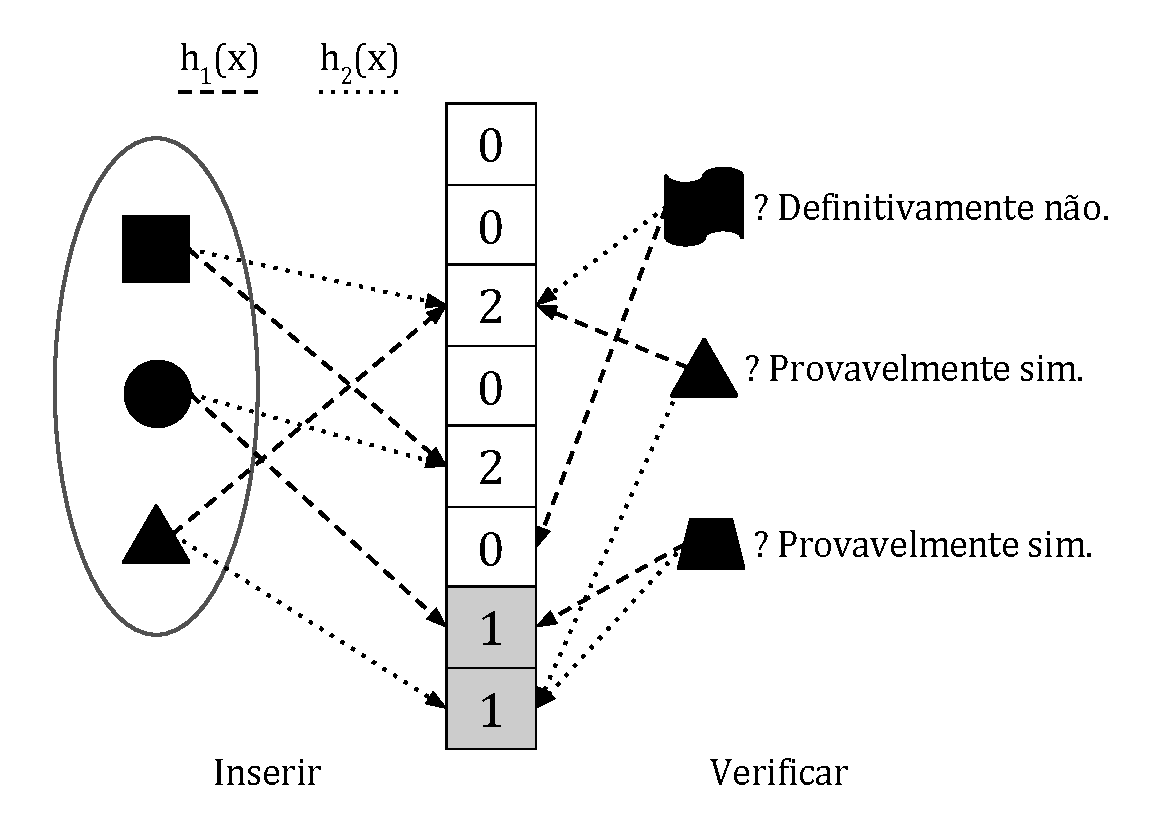
\includegraphics[scale=0.45]{files/bloom2.pdf}
  \caption{Exemplo de filtro de bloom com contagem}
  \label{fig:bloom2}
\end{figure}

A remoção neste filtro baseia-se na ausência de overflows em seus contadores. Para tanto, é preciso dimensionar o tamanho destes contadores de forma a minimizar a probabilidade de overflow. Como originalmente o filtro usa apenas um bit por posição no vetor, qualquer número de bits adicionais escolhidos para representar o contador aumenta significativamente o espaço necessário para armazenar a estrutura. Normalmente, 4 bits são suficientes para a maior parte das aplicações, o que faz com que estes filtros usem quatro vezes mais espaço que filtros normais.

O número de bits por contador determina a probabilidade de \emph{overflow}. \emph{Overflows} em \emph{counting Bloom filters} precisam ser ativamente tratados. Se um \emph{overflow} ocorrer é preciso manter o contador no máximo valor possível. De forma equivalente, ao tentar decrementar uma posição já no maior valor possível, é preciso mantê-la nesse mesmo valor. Faz-se isto para evitar a introdução de falsos negativos.

Na prática, entretanto, \emph{overflows} devem ser consideravelmente raros. A probabilidade de um \emph{overflow} dado que cada contador usa $b$ bits, após inserir $m$ elementos, usando 10 bits por elemento e otimizando o número de funções \emph{hash} é:
\[
Pr[\textsc{overflow}] \leq n \left( \frac{\mathrm{e} \ln 2}{2^b} \right)^{2^b}
\]
como provado por Fan et al. \cite{fan1998summary}. Assim, ao usar 4 bits para os contadores, a probabilidade de overflow concentra-se em:
\[
Pr[\textsc{overflow em 4 bits}] \leq 1.37 \times 10^{-15} \times n
\]

Esta probabilidade baseia-se na possibilidade de produzir funções \emph{hash} realmente aleatórias, o que pode ser aproximado, mas não pode ser garantido. Em um pior caso em especial, se o mesmo elemento for repetidamente oferecido à estrutura, a probabilidade de \emph{overflow} torna-se criticamente alta.

\subsection{Outras variantes}\label{sec:bloom:variants}

O filtro de Bloom, em sua simplicidade, tem limitações que posam como desafios para algumas aplicações. Desde sua concepção, entretanto, muitas extensões foram propostas para superar estas limitações (geralmente em detrimento de algum parâmetro de desempenho), entre elas:

\begin{description}

  \item[\emph{Compressed Bloom Filters} \cite{mitzenmacher2002compressed}] 
    Discute esquemas de compressão para otimizar o tamanho de filtros enviados através de rede ou salvos em disco. O objetivo é construir filtros com mais bits e menos funções \emph{hash}, de forma a minimizar o tamanho comprimido e/ou aumentar a precisão. Especialmente útil em caso de caches distribuídos. 

  \item[\emph{Distance-sensitive Bloom Filters} \cite{kirsch2006distance}] 
    Responde consultas do tipo "algum elemento próximo a $x$ pertence a $S$?", dada uma métrica apropriada, utilizando funções \emph{hash} sensíveis a localidade, com possibilidade tanto de falsos positivos como falsos negativos. Esta variante é bastante útil para detecção de plágio, por exemplo.

  \item[\emph{Dynamic Bloom Filters} \cite{guo2010dynamic}] 
    Permite redimensionar dinamicamente filtros de Bloom sem perder suas propriedades estatísticas. Baseia-se na criação de múltiplos filtros com um limite superior na probabilidade de falsos positivos, i.e., quando um filtro alcança uma taxa de falsos positivos muito alta, outro filtro vazio é criado. Nesta modalidade, a complexidade das operações padrão é maior, entretanto, na prática isso não posa como um problema. É possível dimensionar o tamanho dos filtros a serem criados de forma a amortizar a quantidade de filtros criados ao longo do tempo.

  \item[\emph{Spectral Bloom Filters} \cite{cohen2003spectral}] 
    É uma estrutura especializada em lidar com multiconjuntos. Um \emph{Spectral Bloom Filter} (SBF) funciona praticamente da mesma forma que um \emph{Counting Bloom Filter}, mas suas operações são especializadas em obter a cardinalidade de um certo item num multiconjunto. Nesta estrutura, a cardinalidade de um elemento $x$ se dá por $\displaystyle \min_{i = 1 \dots k} B[h_i(x)]$. A estrutura SBF é conceitualmente similar à \emph{Count-Min}, apresentada na Seção~\ref{sec:countmin}.

\end{description}


\subsection{Aplicações}\label{sec:bloom:apps}

Filtros de Bloom são estruturas simples, porém têm aplicabilidade em muitos domínios diferentes. Eles são especialmente importantes em sistemas que desejam diminuir o custo de verificar se uma operação mais custosa precisa ser feita (como a de determinar se um arquivo está armazenado antes de recorrer ao disco). Estes sistemas estão preparados para lidar com alguns falsos positivos, mas beneficiam-se ao não precisar efetuar tais operações em caso negativo.

\begin{description}

\item[Processadores de texto:]

O artigo original sobre os filtros de Bloom propõe uma aplicação que avalia regras de hifenização \cite{bloom1970space}. Segundo Bloom, no caso descrito, 90\% das regras de hifenização de palavras poderiam ser generalizadas por regras simples e apenas 10\% iriam requerer uma consulta ao disco. Neste caso, um filtro de Bloom seria utilizado para verificar se a palavra é uma das que estão no disco. O falso positivo somente causaria uma ida desnecessária ao disco, o que ainda seria uma vantagem, já que a maioria dos casos poderia ser resolvida em memória.

O mesmo princípio pode ser aplicado para verificação ortográfica. Ramakrishna \cite{ramakrishna1989practical} discute como utilizar filtros de Bloom pode diminuir o espaço necessário para armazenar vários dicionários ao mesmo tempo em memória.

\item[Bancos de dados:]

Há diversas aplicações para filtros de Bloom em bancos de dados. Mullin \cite{mullin1993estimating} descreve um método para estimar o resultado de junções (\emph{joins}) relacionais distribuídos. O filtro é bastante apropriado em sistemas distribuídos, pois diminui a necessidade de comunicação entre os nós para computar alguns resultados. Antognini \cite{antognini2008bloom} mostra usos dos filtros de Bloom no banco de dados Oracle tanto para computar \emph{joins} distribuídos quanto para cache de resultados.

\item[Controle de tráfego de redes:]

Feng et al. \cite{feng1999blue} descrevem uma classe de algoritmos para controle de tráfego de redes conhecido como \textsc{Blue}. Uma das variantes deste algoritmo, conhecida como \textsc{Stochastic Fair Blue} (SFB), estimula um controle de tráfego que pune hosts que congestionam a rede. Muitas vezes o custo de espaço para manter informações sobre esses hosts em memória pode ser impraticável, principalmente considerando a quantidade limitada de recursos em equipamentos de redes. O algoritmo SFB utiliza então um filtro de Bloom para manter estas informações.

\item[Caches distribuídos:]

Em sistemas de cache distribuído é importante que cada nó do cluster possa saber quais chaves seus vizinhos possuem. Uma das técnicas frequentemente empregadas são os \emph{cache digests}, que são uma forma de compressão com perda de todas as chaves presentes em um nó. \emph{Cache digests} usam, entre outras coisas, filtros de Bloom \cite{rousskov1998cache}. Periodicamente os nós trocam \emph{cache digests} entre si para que o conhecimento sobre quais chaves estão em cada um de seus vizinhos seja disseminado. Neste caso, o custo de um falso positivo somente implica em uma requisição a mais para verificar se de fato a chave existe.

\item[Verificação de URLs maliciosas:]

O navegador Google Chrome usa filtros de Bloom para verificar se a \emph{URL} digitada pelo usuário faz parte do banco de dados de sites maliciosos \cite{honoroff2006bloom}. Assim, casos negativos são rapidamente verificados. E na minoria dos casos, quando há um falso positivo, basta uma requisição de rede a mais para retificar a informação.

\end{description}

\subsection{Resultados experimentais}\label{sec:bloom:experiments}

Para melhor observar as previsões teóricas sobre os filtros de Bloom, conduzimos uma série de experimentos com dados reais e sintéticos para verificar empiricamente as probabilidades descritas na teoria. Testamos duas variantes: teste de pertinência com filtro de Bloom clássico e estimativa de cardinalidade com \emph{linear counting}.

Foram utilizados dois conjuntos de dados: um composto por todas as palavras nas obras de Shakespeare (964410 palavras, 23704 distintas) e outro composto por cadeias aleatórias de 32 caracteres (1064960 cadeias no total).

Em todos os testes, a função \emph{hash} utilizada foi MurmurHash 3, de 32 bits.

Com estes dados, foram realizados dois testes: um para observar a quantidade de falsos positivos e outro para observar o desvio entre a cardinalidade estimada e a real. Os filtros de Bloom foram dimensionados de acordo com cada conjunto de dados, como descrito na Tabela~\ref{table:bloom_test_setup}. Para ambos os conjuntos de dados, foram utilizadas 7 funções \emph{hash} no filtro para falsos positivos.

\begin{table}[!htbp]
\begin{center}
	\begin{tabular}{ c | c | c }
		\hline 
		& {\bf Shakespeare} & {\bf Cadeias aleatórias} \\
		\hline 
		{\bf filtro para falsos positivos} & 16384 bits & 1048576 bits \\
		{\bf filtro para cardinalidade} & 2048 bits & 131072 bits \\
		{\bf palavras inseridas} & 20000 & 1048576 \\
		{\bf palavras verificadas} & 3704 & 16384 \\
		\hline 
	\end{tabular}
	\caption{Configuração dos filtros de teste}
	\label{table:bloom_test_setup}
\end{center}
\end{table}

Durante a inserção das palavras, a cada 2.5\% de palavras inseridas, o teste era realizado: no caso dos falsos positivos, o conjunto de verificação era executado contra o filtro verificando a porcentagem de falsos positivos; no caso do teste de cardinalidade, estimando a cardinalidade e registrando a razão entre esta e a cardinalidade real do conjunto até o momento.

Como os dois testes foram realizados com conjuntos de tamanhos diferentes, todos os resultados serão apresentados aqui em valores relativos de fator de carga.

No teste de falsos positivos, como pode ser visto na Figura~\ref{fig:bloom_test_falsep}, a quantidade dos mesmos ficou extremamente aderente à teoria. É possível perceber como o fator de carga sozinho é capaz de influenciar a probabilidade de falsos positivos. O valor esperado neste teste é o mesmo descrito na Seção~\ref{sec:bloom:false}.

\begin{figure}[!htbp]
\centering
\scalebox{0.80}{\begin{tikzpicture}[
        declare function = {
            p(\n,\m,\k) = ((1 - (e^(-\k*\n/\m)))^\k);
        }
    ]
	\begin{axis}[
	    scaled ticks=false, 
        grid=both,
        xlabel=load factor ($n/m$),
		ylabel=falsos positivos,
		yticklabel=\pgfmathparse{100*\tick}\pgfmathprintnumber{\pgfmathresult}\,\%,
		xticklabel=\pgfmathparse{100*\tick}\pgfmathprintnumber{\pgfmathresult}\,\%,
		ymin=0, ymax=1,
		xmin=0, xmax=1, 
		legend columns=1, 
	    legend style={legend pos=outer north east,}
    ]
    
    \addplot[line width=15pt,domain=0:1,samples=30,color={rgb:black,1;white,1},opacity=0.4]{p(x*16384,16384,7)};
	\addplot[mark=*,black,mark options={scale=0.75}] table[x=n_member,y=p_member] {files/bloom_shakespeare.txt};
	\addplot[mark=o,black,mark options={scale=0.75}] table[x=n_member,y=p_member] {files/bloom_random.txt};
	\legend{esperado, shakespeare, aleatório};

	\end{axis}
\end{tikzpicture}}
\caption{Falsos positivos observados e probabilidade esperada.}
\label{fig:bloom_test_falsep}
\end{figure}

Para o teste de cardinalidade foram utilizados filtros com uma quantidade de bits menor, para poder observar fatores de carga maiores que $ 100\%$. O resultado pode ser visto na Figura~\ref{fig:bloom_test_cardinality}. É possível perceber que aumentando o tamanho do filtro ($m$) a precisão aumenta, mesmo quando comparado em termos relativos de fator de carga.

\begin{figure}[!htbp]
\centering
\scalebox{0.80}{\begin{tikzpicture}[
        declare function = {
            p(\n,\m) = max(min(2*(\m*(e^(\n/\m) - (\n/\m) - 1)) ^ (1/2) / (\n), 0.1), -0.1);
        }
    ]
	\begin{axis}[
        title={shakespeare},
	    scaled ticks=false, 
        grid=both,
        xlabel=load factor ($n/m$),
		ylabel=erro ($\hat{n}/n-1$),
		yticklabel=\pgfmathparse{100*\tick}\pgfmathprintnumber{\pgfmathresult}\,\%,
		xticklabel=\pgfmathparse{100*\tick}\pgfmathprintnumber{\pgfmathresult}\,\%,
		ymin=-0.1,ymax=0.1,ystep=0.02,
		xmin=0, xmax=8, 
		legend columns=1, 
    ]
    
    \addplot[line width=15pt,domain=0:1,samples=30,color={rgb:black,1;white,1},opacity=0.4]{2};

    \addplot[name path=line3, line width=0pt,domain=0:8,samples=60,opacity=0.0,forget plot]{p(x*4096,4096)};
    \addplot[name path=line4, line width=0pt,domain=0:8,samples=60,opacity=0.0,forget plot]{-p(x*4096,4096)};
	\addplot[fill={rgb:black,1;white,1},fill opacity=0.40,forget plot] fill between[ of = line3 and line4];

	\addplot[mark=*,black,smooth,mark options={scale=0.75}] table[x=n_count,y=p_count] {files/bloom_shakespeare.txt};

	\end{axis}
\end{tikzpicture} \begin{tikzpicture}[
        declare function = {
            p(\n,\m) = max(min(2*(\m*(e^(\n/\m) - (\n/\m) - 1)) ^ (1/2) / (\n), 0.1), -0.1);
        }
    ]
	\begin{axis}[
	    title={aleatório},
	    scaled ticks=false, 
        grid=both,
        xlabel=load factor ($n/m$),
		yticklabel=\pgfmathparse{100*\tick}\pgfmathprintnumber{\pgfmathresult}\,\%,
		xticklabel=\pgfmathparse{100*\tick}\pgfmathprintnumber{\pgfmathresult}\,\%,
		ymin=-0.1,ymax=0.1,ystep=0.02,
		xmin=0, xmax=8, 
		legend columns=1, 
    ]
    
    \addplot[line width=15pt,domain=0:1,samples=30,color={rgb:black,1;white,1},opacity=0.4]{2};

    \addplot[name path=line1, line width=0pt,domain=0:8,samples=60,opacity=0.0,forget plot]{p(x*131072,131072)};
    \addplot[name path=line2, line width=0pt,domain=0:8,samples=60,opacity=0.0,forget plot]{-p(x*131072,131072)};
	\addplot[fill={rgb:black,1;white,1},fill opacity=0.40,forget plot] fill between[ of = line1 and line2];

	\addplot[mark=*,black,smooth,mark options={scale=0.75}] table[x=n_count,y=p_count] {files/bloom_random.txt};
	\legend{esperado, observado};

	\end{axis}
\end{tikzpicture}}
\caption{Erro observado por funções \emph{hash}}
\label{fig:bloom_test_cardinality}
\end{figure}

Na figura, o erro esperado é apresentado no valor de 2 erros padrão, desta forma, espera-se que aproximadamente 95\% das estimativas estejam dentro deste erro.

Apesar do teste apresentar uma flutuação maior no resultado, observa-se com clareza como a estimativa de cardinalidades continua com resultados satisfatórios (erro menor que 10\%) para fatores de carga muito maiores que 100\%.
%~~~~~~~~~~~~~~~~~~~~~~~~~~~~~~~~~~~~~~~~~~~~~~~~~~~~~~~~~~~~~~~~~~~~~~~
\section{\emph{Count-Min Sketch}}\label{sec:countmin}
%~~~~~~~~~~~~~~~~~~~~~~~~~~~~~~~~~~~~~~~~~~~~~~~~~~~~~~~~~~~~~~~~~~~~~~~

\emph{Count-Min Sketch} é uma estrutura probabilística, descrita por Cormode e Muthukrishnan \cite{cormode2005improved}, que permite representar um vetor implicitamente e incrementalmente e estimar consultas sobre ele. 

Esta estrutura mostra-se importante em casos onde o vetor representado não caberia em memória, sendo aceitáveis resultados probabilísticos para consultas específicas.

Em especial, \emph{Count-Min Sketch} e suas variantes permitem estimar o valor em índices e intervalos específicos do vetor, bem como o produto escalar entre diferentes vetores.

Estas operações ajudam a resolver muitos problemas relacionados à análise de fluxos de dados. Em especial, ao representar os elementos de um multiconjunto de inteiros como os índices do vetor $A$, e suas frequências como os valores, é possível utilizar a consulta de intervalo para estimar os percentis do multiconjunto original.

\subsection{Definição}


O objetivo de \emph{Count-Min Sketch} é representar um vetor $A$,  definido incrementalmente através de operações de atualização na forma de pares ordenados $(i, c)$, que representam um acréscimo de $c$ unidades na i-ésima posição do vetor. Isto é $A[i] \gets A[i] + c$. 

O vetor e suas atualizações não precisam ser mantidos em memória. A estrutura permite a qualquer momento, efetuar consultas sobre parâmetros do vetor original, respondidas probabilisticamente. Em especial, descreveremos nesta seção o processo para responder as seguintes consultas:

\begin{itemize}
  \item Para um índice $i$, o valor $A[i]$;
  \item Para vetores $A$ e $B$, o produto escalar $A \cdot B$.
\end{itemize}

\emph{Count-Min Sketch} funciona de forma similar a um filtro de Bloom com contagem, entretanto, em vez de apenas um vetor, a estrutura utiliza uma matriz $M[1..m, 1..k]$, onde cada coluna corresponde a uma função \emph{hash}.

A atualização parte de um par ordenado $(i, c)$, representando um incremento de valor $c$ na $i$-ésima posição do vetor implícito $A$. O algoritmo consiste em incrementar na matriz todas as posições referenciadas pelos hashs calculados em cada um dos seus respectivos vetores (Algoritmo~\ref{alg:countminupdate}). 

\begin{algorithm}
\linespread{1}\selectfont
\caption{Atualiza Count-Min}
\label{alg:countminupdate}
\begin{algorithmic}[1]
\Procedure{Atualizar}{$i$, $c$}
    \For{$j \gets  1 \textrm{ to } k$}
        \State $M[h_j(i), j] \gets M[h_j(i), j] + c$
	\EndFor
\EndProcedure
\end{algorithmic}
\end{algorithm}

A consulta por valor se dá obtendo o mínimo entre todas as células referenciadas pelas funções \emph{hash}  (Algoritmo~\ref{alg:countminquery}).

\begin{algorithm}
\linespread{1}\selectfont
\caption{Estima valor de $A[i]$}
\label{alg:countminquery}
\begin{algorithmic}[1]
\Function{Estimar}{$i$}
    \State $resultado \gets \infty$ 
    \For{$j \gets  1 \textrm{ to } k$}
        \State $resultado \gets \min(resultado, M[h_j(i), j])$
	\EndFor
	\Return $resultado$
\EndFunction
\end{algorithmic}
\end{algorithm}

A Figura~\ref{fig:countmin1} exemplifica os dois processos anteriores.

\begin{figure}[!htbp]
  \centering
  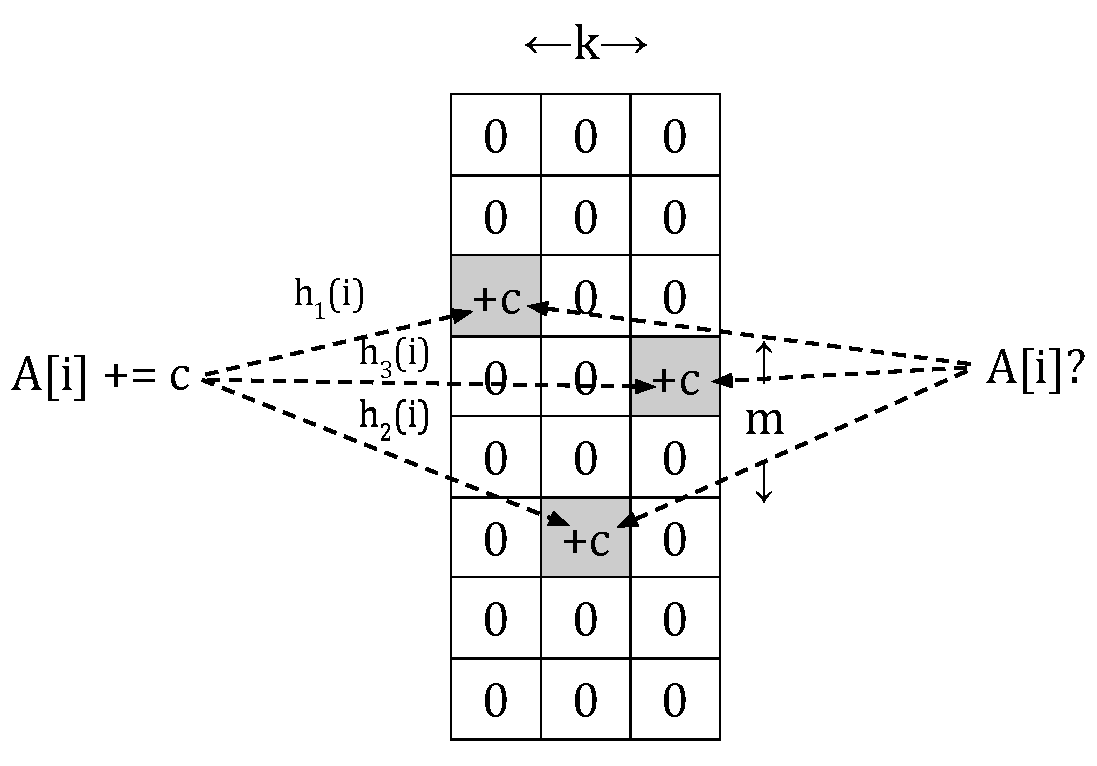
\includegraphics[scale=0.45]{files/countmin1.pdf}
  \caption{Atualização e consulta em um \emph{Count-Min Sketch}}
  \label{fig:countmin1}
\end{figure}

Percebe-se intuitivamente que, no caso de $\forall_i A[i] \leq 0$ no momento da consulta, o valor estimado pela mesma nunca é menor do que o valor real do elemento, isto é: $A[i] \leq \widehat{A[i]}$. Este resultado é importante, pois representa muitos casos reais de uso, como contagem de acessos de usuários ou monitoramento de uso e liberação de recursos compartilhados.

Dadas duas matrizes \emph{Count-Min} $M_A[1..m, 1..k]$ e $M_B[1..m, 1..k]$ representando, respectivamente, vetores implicitos $A$ e $B$, é possível estimar o produto escalar $A \cdot B$ obtendo o mínimo valor entre os produtos escalares das respectivas colunas nas duas matrizes, como mostrado no Algoritmo~\ref{alg:countminscalar}.

\begin{algorithm}
\linespread{1}\selectfont
\caption{Estima $A \cdot B$}
\label{alg:countminscalar}
\begin{algorithmic}[1]
\Function{Produto-Escalar}{$M_A$, $M_B$}
    \State $resultado \gets \infty$ 
    \For{$i \gets  1 \textrm{ to } k$}
        \State $soma \gets 0$ 
        \For{$j \gets  1 \textrm{ to } m$}
            \State $soma \gets soma + M_A[i, j] \cdot M_B[i, j]$
        \EndFor
        \State $resultado = \min(resultado, soma)$
	\EndFor
	\Return $resultado$
\EndFunction
\end{algorithmic}
\end{algorithm}

De forma análoga à consulta pontual, caso ambos os vetores tenham apenas elementos não-negativos, vale que $A \cdot B \leq \widehat{A \cdot B}$.

\subsection{Exemplo}\label{sec:countmin:example}


\subsection{Estimativa do erro}

Em \cite{cormode2005improved} é mostrado que a escolha dos parâmetros $m$ e $k$ se dá de forma a definir $\epsilon$ (o fator de erro) e $\delta$ (a confiança do erro). Isto é, dados $m = \lceil e/\epsilon \rceil$ e $k = \lceil \ln(1/\delta) \rceil$, é possível mostrar que o erro da estimativa $\widehat{A[i]}$ se dá por um fator de $\epsilon$. Mais especificamente, se $\forall_i A[i] \geq 0$,
\[
A[i] \leq \widehat{A[i]} \leq A[i] + \epsilon \lVert A \rVert_1
\]
com probabilidade inferior a $1 - \delta$.

Para demonstrar este resultado, precisamos introduzir uma variável aleatória $I_{h,i,j}$, que representa, para cada função \emph{hash}, incidência de dois índices distintos em $A$ na mesma linha na matriz. Isto é, para cada função $h$
\[
    I_{h,i,j} = \begin{cases} 
        1 & \text{se}\ i \neq j \wedge h(i) = h(j) \\
        0 & \text{caso contrário} \\
    \end{cases}
\]

Perceba que $I_{h,i,j}$ é uma variável de Bernoulli, portanto, 
\[
\text{E}[I_{h,i,j}] = \Pr[h(i) = h(j)] = \frac{1}{m} \leq \frac{\epsilon}{e}
\]

Definimos também uma variável $X_{h, i}$, que representa, para cada função \emph{hash}, o somatório de elementos em $A$ (exceto o próprio índice $i$) que foram adicionados na mesma célula da matriz que $A[i]$, isto é
\[
    X_{h, i} = \sum_{j=1}^{n} I_{h,i,j} A[j]
\]

A variável $X_{h, i}$ pode ser interpretada como o erro na estimativa para cada função \emph{hash}, isto é $M[h_q(i), q] = A[i] + X_{h_q, i}$. Como todo $A[i]$ é não-negativo, $X_{h, i}$ também é não-negativo, portanto $\widehat{A[i]} \geq A[i]$. Além disso, pela linearidade da expectativa, 
\[
    \text{E}[X_{h, i}] = \text{E} \left[ \sum_{j=1}^{n} I_{h,i,j} A[j] \right] =  \text{E}[I_{h,i,j}] \sum_{j=1}^{n}A[j] \leq \frac{\epsilon}{e} \lVert A \rVert_1
\]

Para provar o limite superior, analisaremos a probabilidade de uma estimativa estar acima deste limite. Para isso, todas as funções \emph{hash} precisam gerar estimativas acima do limite, ou seja
\begin{align*}
    \Pr\left[ \widehat{A[i]} > A[i] + \epsilon \lVert A \rVert_1\right] 
    &= \Pr\left[ \forall_q^k M[h_q(i), k] > A[i] + \epsilon \lVert A \rVert_1 \right] \\
    &= \Pr\left[ \forall_q^k A[i] + X_{h_q,i} > A[i] + \epsilon \lVert A \rVert_1 \right] \\
    &= \Pr\left[ \forall_q^k X_{h_q,i} > e \text{E} [X_{h_q,i}] \right] \\
    &= (\Pr\left[ X_{h_q,i} > e \text{E} [X_{h_q,i}] \right])^k
\end{align*}
e, pela desigualdade de Markov,
\[
    \Pr\left[ \widehat{A[i]} > A[i] + \epsilon \lVert A \rVert_1 \right] < \frac{1}{e^k} \leq \delta \\
\]

Ou seja, para o caso $\forall_i A[i] \geq 0$, a probabilidade da estimativa $\widehat{A[i]}$ não ultrapassar o limite superior definido é menor que $1 - \delta$.

É possível utilizar uma variante do algoritmo para o caso geral, onde $A[i]$ pode assumir valores negativos no momento da estimativa. Neste caso, utiliza-se a mediana como estimativa no lugar do mínimo. É possível então demonstrar que
\[
A[i] - 3 \epsilon \lVert A \rVert_1 \leq \widehat{A[i]} \leq A[i] + 3 \epsilon \lVert A \rVert_1
\]
com probabilidade $1 - \delta^{1/4}$. Basta observar que dado que $M[h_q(i), q] = A[i] + X_{h_q, i}$, segue
\[
\text{E}\left[ |M[h_q(i), q] - A[i]| \right] = \text{E}[X_{h_q,i}] \leq \frac{\epsilon}{e} \lVert A \rVert_1
\]

Aplicando novamente a desigualdade de Markov, mostra-se que a probabilidade da estimativa de cada função \emph{hash} estar errada por um valor absoluto maior que $3\epsilon \lVert A \rVert_1$ é menor que $1/3e$. Como estamos obtendo a mediana de $\lceil \ln(1/\delta) \rceil$ estimadores, a probabilidade de pelo menos metade deles estar acima do limite de erro que pretendemos provar, pelo limite de Chernoff, é menor que $\delta^{1/4}$.

Por fim, o erro esperado para a estimativa do produto escalar entre vetores se dá pela desigualdade
\[
    A \cdot B \leq \widehat{A \cdot B} \leq A \cdot B + \epsilon \lVert A \rVert_1 \lVert B \rVert_1
\]

Para esta demonstração, definimos $(\widehat{A \cdot B})_q$ como a estimativa do produto escalar considerando apenas a coluna $q$ da matriz. Pela construção da matriz, pode-se dizer que
\[
    (\widehat{A \cdot B})_q = A \cdot B + \sum_{i,j} I_{h_q,i,j} \cdot A[i] \cdot B[j] 
\]

Como todo ambos $A$ e $B$ possuem apenas elementos não-negativos, é fácil mostrar que tanto os valores de $(\widehat{A \cdot B})_q$ como a estimativa final (por consequência) são maiores que o valor do produto escalar $A\cdot B$. Além disso,
\begin{align*}
    E\left[ (\widehat{A \cdot B})_q - A \cdot B \right] 
    &= E\left[ \sum_{i,j} I_{h_q,i,j} \cdot A[i] \cdot B[j]  \right] \\
    &= \sum_{i,j} E\left[ I_{h_q,i,j} \right] \cdot A[i] \cdot B[j] \\
    &\leq \frac{\epsilon}{e}   \lVert A \rVert_1 \lVert B \rVert_1
\end{align*}

Assim, a probabilidade de todas as funções \emph{hash} produzirem estimativas acima do limite é dada por
\begin{align*}
    \Pr\left[ \widehat{A \cdot B} > A \cdot B + \epsilon \lVert A \rVert_1 \lVert B \rVert_1 \right] 
    &= \Pr\left[ \forall_q^k (\widehat{A \cdot B})_q -  A \cdot B > \epsilon \lVert A \rVert_1 \lVert B \rVert_1 \right] \\
    &= \Pr\left[ \forall_q^k (\widehat{A \cdot B})_q -  A \cdot B > e  E\left[ (\widehat{A \cdot B})_q - A \cdot B \right]  \right] \\
    &= \left(\Pr\left[ (\widehat{A \cdot B})_q -  A \cdot B > e  E\left[ (\widehat{A \cdot B})_q - A \cdot B \right]  \right]\right)^k \\
\end{align*}

logo, utilizando a desigualdade de Markov,
\[
    \Pr\left[ \widehat{A \cdot B} > A \cdot B + \epsilon \lVert A \rVert_1 \lVert B \rVert_1 \right] < \frac{1}{e^k} \leq \delta \\
\]

Perceba que este é um resultado compatível e mais geral à consulta de ponto no vetor. Neste caso, bastaria utilizar um vetor $B$, com apenas o índice $i$ contendo o valor $1$. Assim, o produto escalar deste com um vetor $A$ arbitrário seria equivalente a obter $A[i]$.

\subsection{Consultas de intervalo}

É possível utilizar \emph{Count-Min Sketch} para consultas de intervalo $Q(a, b) = \sum_{i=a}^b A[i]$ em um vetor $A[0..n-1]$. A ideia trivial seria fazer a estimativa de todos os valores $A[i]$ no intervalo selecionado. Porém, esta estratégia acumula erro proporcional ao tamanho do intervalo.

Uma outra estratégia envolve manter não apenas um, mas $\log_2 n$ matrizes $M_y, 0 \leq y < \log_2 n$, representando implicitamente vetores $A_y$, onde cada $A_y[i] = \sum_{j=0}^{2^y-1} A[i+j]$. Isto permite que qualquer consulta nos intervalos em $[0, n)$ seja efetuada com no máximo $2 \log_2 n$ consultas nas matrizes subjacentes. A Figura~\ref{fig:countmin2} exemplifica uma dessas consultas.

\begin{figure}[!htbp]
  \centering
  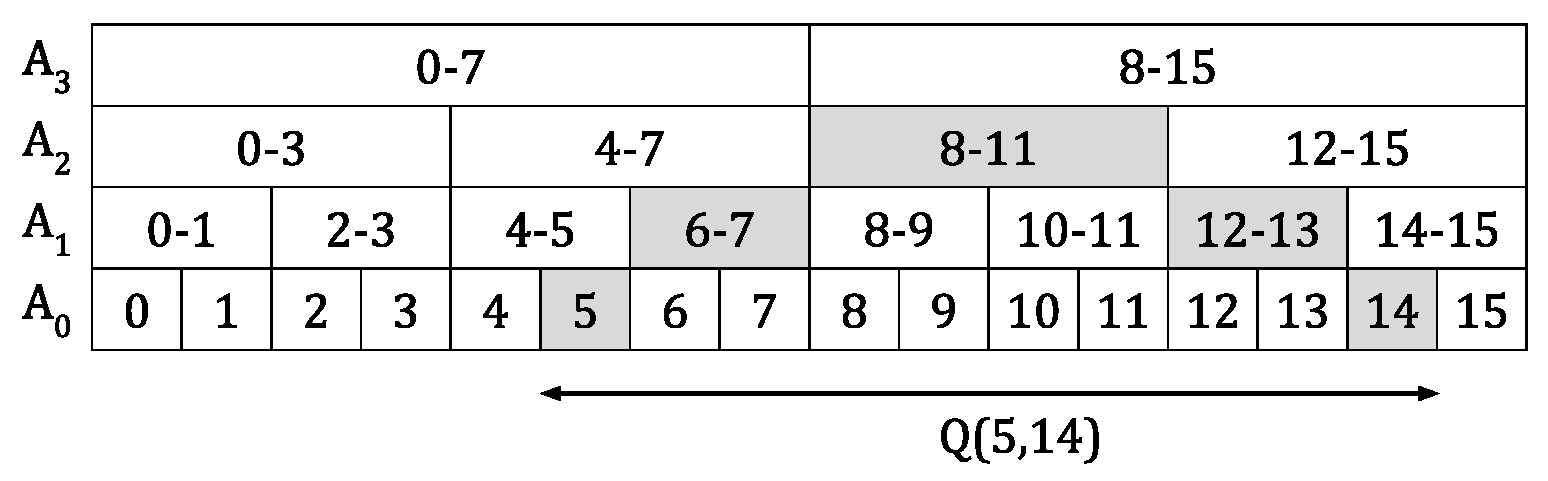
\includegraphics[scale=0.45]{files/countmin2.pdf}
  \caption{Consulta de intervalo $Q(5, 14)$ para $n=16$}
  \label{fig:countmin2}
\end{figure}

A atualização envolve em, ao receber uma tupla $(i, c)$, atualizar cada uma das matrizes. Porém o índice utilizado em cada matriz é diferente. Seja $i_y$ o índice usado para atualizar a matriz $M_y$, todos os bits $i_y$ deve ser iguais aos de $i$, exceto os $y$ últimos, que devem ser zero.

Por exemplo, para atualizar $i=7$ num vetor com $n=16$, as seguinte posições devem ser atualizadas nos vetores implícitos: $i_0 = 7$, $i_1=6$, $i_2=4$ e $i_3=0$. O Algoritmo~\ref{alg:countminrangeupdate} mostra como se dá essa atualização.

\begin{algorithm}
\linespread{1}\selectfont
\caption{Atualiza Count-Min para busca por intervalo}
\label{alg:countminrangeupdate}
\begin{algorithmic}[1]
\Procedure{Atualizar}{$i$, $c$}
    \For{$y \gets 0 \textrm{ to } \log_2 n - 1$}
        \State $i_y \gets i \textrm{ com os } y \textrm{ bits menos significativos desligados}$
        \For{$j \gets  1 \textrm{ to } k$}
            \State $M_y[h_j(i_y), j] \gets M_y[h_j(i_y), j] + c$
    	\EndFor
	\EndFor
\EndProcedure
\end{algorithmic}
\end{algorithm}

A consulta envolve decidir e estimar os valores para os sub-intervalos canônicos que compõem o intervalo de busca. A decomposição em sub-intervalos canônicos pode ser feita de forma gulosa, em cada passo procurando o maior sub-intervalo que seja prefixo do intervalo atual. Para os fins do algoritmo, o mais importante é encontrar qual vetor $A_y$ representa o intervalo em questão. O Algoritmo~\ref{alg:countminrangequery} mostra como funciona o processo de consulta.

\begin{algorithm}
\linespread{1}\selectfont
\caption{Estima o somatório dos elementos no intervalo}
\label{alg:countminrangequery}
\begin{algorithmic}[1]
\Function{Estimar-Intervalo}{$a$, $b$}
    \State $soma \gets 0$
    \While{$a \leq b$}
        \State $y \gets $ maior índice de vetor $A_y$ que representa algum prefixo de $[a, b]$.
        \State $minimo \gets \infty$
        
        \For{$j \gets  1 \textrm{ to } k$}
            \State $minimo \gets \min(minimo, M_y[h_j(a), j])$
    	\EndFor
    	
    	\State $soma \gets soma + minimo$
    	\State $a \gets a + 2^y$
    \EndWhile
    \Return $soma$
\EndFunction
\end{algorithmic}
\end{algorithm}

Ainda seguindo o trabalho em \cite{cormode2005improved}, é possível mostrar que o erro desta estimativa é dado por
\[
    A[a..b] \leq \widehat{A[a..b]} \leq A[a..b] + 2  \epsilon \log_2 n \lVert A \rVert_1
\]
com probabilidade $1-\delta$.

O princípio que rege este erro é o mesmo da consulta pontual. Neste caso, a ideia é mostrar que o erro de cada estimativa (somatório de até $2\log_2 n$ observações independentes de $X_{h,i}$) tem valor esperado $2 \log_2 n (\epsilon/e) \lVert A \rVert_1$. Assim, aplicando a mesma desigualdade de Markov temos o resultado descrito acima. 

É importante notar que na prática, o erro pode ser menor para intervalos cujos limites possuam um número menor de bits ligados, pois seriam necessários menos sub-intervalos para compor o intervalo da consulta.

\subsection{Aplicações}

A estrutura \emph{Count-Min Sketch} permite a representação de vetores arbitrários sem o custo de mantê-los inteiramente em memória. Isto pemite a utilização de diversos algoritmos clássicos que seriam custosos em uma situação de restrição de recursos, mas que não sofreriam tanto em trocar acurácia das respostas por um uso mais controlado de memória.

\begin{description}

\item[Bioinformática:]

Em \cite{zhang2014these} é mostrado um caso onde a estrutura \emph{Count-Min sketch} é usada para manter a contagem de \emph{k-mers} (subsequências de K bases nitrogenadas em sequências de DNA). Estas frequências são usadas para alimentar outros algoritmos, que passam então a atuar de forma probabilística. O uso de estruturas probabilísticas neste caso é importante para aliviar o uso de memória para representar conjuntos de dados que não raramente chegam a dezenas de bilhões de registros.

\item[Segurança:]

Muitos equipamentos de segurança possuem uma quantidade limitada de recursos computacionais. Isto torna atrativo o uso de estruturas de \emph{sketch} para manter informações críticas em tempo real. Em \cite{salem2008novel} é descrito um mecanismo que usa \emph{Count-Min sketch} para verificar se uma certa combinação de parâmetros de conexão exibe uma frequência muito superior à média, o que pode ser um sinal de ataque.

Além disso, em \cite{schechterpopularity}, pesquisadores da Microsoft apresentam um mecanismo para manter uma estrutura com a frequência de senhas para invalidar senhas muito comuns, aumentando a segurança dos sistemas. A vantagem de usar \emph{Count-Min} neste caso é capacidade de armazenar a frequência de uma senha sem manter a senha em si na estrutura.

\item[Bancos de Dados:]

Um uso prático para a estrutura \emph{Count-Min sketch} é a estimativa de joins relacionais em bancos distribuídos \cite{cormode2005improved,rusu2007statistical}. Neste uso, seria computada a estrutura para o vetor de frequências dos diferentes valores que um certo atributo pode ter e, apenas transferindo o \emph{sketch} é possível estimar a cardinalidade do join, através da estimativa do produto escalar entre os dois vetores.

\item[Sistemas distribuídos:]

Encontrar certos elementos muito frequentes num fluxo de dados tem muitas aplicações práticas, como detecção de cenários de erros persistentes. Entretanto, algoritmos determinísticos para esse problema geralmente envolvem manter um contador para cada elemento distinto no conjunto. Utilizando a estrutura \emph{Count-Min sketch} é possível derivar um algoritmo que estima com alta probabilidade quais são os elementos mais frequentes \cite{zhao2006finding}. Este algoritmo ainda tem a vantagem de poder ser executado de forma distribuída, pela própria natureza da estrutura de dados.




\end{description}

\subsection{Resultados experimentais}\label{sec:count:experiments}

Com o objetivo de testar as previsões teóricas sobre a estrutura \emph{Count-Min sketch}, realizamos experimentos que verificam empiricamente os erros descritos anteriormente.

Cada teste usou uma variação do mesmo conjunto de daods composto por todas as obras de Shakespeare (42 obras, 964410 palavras, 23704 distintas). Em todos os casos, a família de funções \emph{hash} utilizada foi MurmurHash 3 \cite{appleby2012murmur}, de 32 bits. Várias funções foram geradas, usando sementes diferentes. Para todos os testes, fixamos $k=3$, o que resulta em uma confiança acima de 95\% para todas as estimativas

No primeiro teste, todas as palavras em todas as obras foram inseridas em \emph{sketches} com $m$ variando entre 128 e 4096. Depois, foram estimados as frequências de cada uma das palavras distintas bem como o erro relativo à norma $\lVert A \rVert_1$ do vetor. O resultado (média e percentil 99), bem como a previsão teórica, podem ser observado na Figura~\ref{fig:countmin_result}.

\begin{figure}[!htbp]
\centering
\scalebox{0.80}{\begin{tikzpicture}[
            declare function = {
                p(\m) = min(e/\m, 0.01);
            }
        ]
    	\begin{axis}[
    	    %height=7cm, width=13cm,
    	    scaled ticks=false, 
            grid=both,
            ylabel={erro relativo a $\lVert A \rVert_1$},
            xlabel=tamanho de cada vetor ($m$),
    		yticklabel=\pgfmathparse{100*\tick}\pgfmathprintnumber{\pgfmathresult}\,\%,
    		ymin=0,ymax=0.003,
    		xmin=0, xmax=4096, 
    		legend columns=1, 
    		legend style={legend pos=outer north east,}
        ]
    
        \addplot[line width=15pt,domain=0:1,samples=30,color={rgb:black,1;white,1},opacity=0.4]{0.01};
    
        \addplot[name path=line3, line width=0pt,domain=1:4096,samples=40,opacity=0.0,forget plot]{p(x)};
        \addplot[name path=line4, line width=15pt,domain=1:4096,samples=30,opacity=0.0, forget plot]{0};
    
    	\addplot[fill={rgb:black,1;white,1},fill opacity=0.40,forget plot] fill between[ of = line3 and line4];
    
    	\addplot[line width=1pt, mark=*,black,smooth, mark options={scale=0.75}] table[x=k,y=mean] {files/countmin.txt};
    	\addplot[dashed,line width=1pt, mark=none,black,smooth, mark options={scale=0.75}] table[x=k,y=p99] {files/countmin.txt};
    	\legend{esperado ($\delta = 0.05$), observado (média), observado ($P_{99}$)};

    	\end{axis}
    \end{tikzpicture}}
\caption{Distribuição de similaridades entre pares de documentos}
\label{fig:countmin_result}
\end{figure}

O segundo teste agrupo os textos por obra, em um total de 42 obras. Para cada obra, foi feita uma cópia deste conjunto com uma certa porcentagem aleatória de palavras substituídas por strings aleatórias. 84 conjuntos de palavras foram utilizados no total.

Para cada conjunto de palavras foram computados \emph{Count-Min sketches} do vetor de frequências com $m$ variando entre 128 e 4096. Para cada par de conjuntos, foi estimado o produto escalar e seu erro (relativo a $\lVert A \rVert_1 \cdot \lVert B \rVert_1$). O resultado (média e percentil 99) pode ser observado na Figura~\ref{fig:countmin_product_result}.

\begin{figure}[!htbp]
\centering
\scalebox{0.80}{\begin{tikzpicture}[
            declare function = {
                p(\m) = min(e/\m, 0.01);
            }
        ]
    	\begin{axis}[
    	    %height=7cm, width=13cm,
    	    scaled ticks=false, 
            grid=both,
            ylabel={erro relativo a $\lVert A \rVert_1 \cdot \lVert B \rVert_1$},
            xlabel=tamanho de cada vetor ($m$),
    		yticklabel=\pgfmathparse{100*\tick}\pgfmathprintnumber{\pgfmathresult}\,\%,
    		ymin=0,ymax=0.003,
    		xmin=0, xmax=4096, 
    		legend columns=1, 
		    legend style={legend pos=outer north east,}
        ]
    
        \addplot[line width=15pt,domain=0:1,samples=30,color={rgb:black,1;white,1},opacity=0.4]{0.01};
    
        \addplot[name path=line3, line width=0pt,domain=1:4096,samples=40,opacity=0.0,forget plot]{p(x)};
        \addplot[name path=line4, line width=15pt,domain=1:4096,samples=30,opacity=0.0, forget plot]{0};
    
    	\addplot[fill={rgb:black,1;white,1},fill opacity=0.40,forget plot] fill between[ of = line3 and line4];
    
    	\addplot[line width=1pt, mark=*,black,smooth, mark options={scale=0.75}] table[x=k,y=mean] {files/countmin_product.txt};
    	\addplot[dashed,line width=1pt, mark=none,black,smooth, mark options={scale=0.75}] table[x=k,y=p99] {files/countmin_product.txt};
    	\legend{esperado ($\delta = 0.05$), observado (média), observado ($P_{99}$)};

    	\end{axis}
    \end{tikzpicture}}
\caption{Distribuição de similaridades entre pares de documentos}
\label{fig:countmin_product_result}
\end{figure}

Estes resultados mostram que os limites teóricos calculados são relativamente conservadores, o que pode ser explicado pelo uso da desigualdade de Markov, que impõe um limite fraco sobre a probabilidade de dispersão.

%~~~~~~~~~~~~~~~~~~~~~~~~~~~~~~~~~~~~~~~~~~~~~~~~~~~~~~~~~~~~~~~~~~~~~~~
\section{\emph{MinHash}}\label{sec:minhash}
%~~~~~~~~~~~~~~~~~~~~~~~~~~~~~~~~~~~~~~~~~~~~~~~~~~~~~~~~~~~~~~~~~~~~~~~

\emph{MinHash} é um algoritmo \emph{hash}ing sensível a localização que permite estimar a semelhança entre conjuntos de forma indireta, através da aproximação do coeficiente de similaridade de \emph{Jaccard}. 

O algoritmo foi inventado por Andrei Broder \cite{broder1997resemblance} como forma de detectar páginas quase-duplicadas no mecanismo de busca Alta Vista. Antes disso, Heintze \cite{heintze1996scalable} e Manber \cite{manber1994finding} já haviam descrito um mecanismo de \emph{fingerprinting} de documentos para rápida indexação e busca por similaridade.  Entretanto, somente com o artigo de Broder, a técnica ganhou mais notoriedade.

\emph{MinHash} possui muitas aplicações. A principal envolve a detecção de documentos quase duplicados, através da representação dos mesmos como o conjunto de palavras ou n-gramas que contêm. O algoritmo, entretanto, possui aplicações diversas, desde sistemas de recomendação \cite{das2007google} até técnicas processamento de som \cite{chiu2010background,covell2007known}.

\subsection{Definição}

O objetivo do algoritmo \emph{MinHash} é estimar o coeficiente de Jaccard. Este coeficiente é definido, para dois conjuntos $A$ e $B$, como a razão entre a cardinalidade da interseção e a cardinalidade da união dos conjuntos \cite{real1996probabilistic}.
\[
J(A, B) = \frac{| A \cap B |}{| A \cup B|}
\]

O coeficiente $J(A, B)$ assume valores entre 0 e 1, sendo 0 para $A$ e $B$ disjuntos e 1 para $A$ e $B$ idênticos. Por exemplo, para os conjuntos:
\[
\begin{split}
A &= \{1, 3, 7, 14, 20\}\ \text{e} \\
B &= \{1, 3, 7, 19, 20, 35\}\text{,}
\end{split}
\]

o valor do coeficiente é:
\[
J(A, B) = \frac{ |\{1, 3, 7, 20 \}| }{ |\{1, 3, 7, 14, 19, 20, 35\}| } = \frac{4}{7} = 0.571428\dots
\]

Embora seja trivial calcular o coeficiente de \emph{Jaccard}, pode ser computacionalmente custoso realizar a comparação entre muitos pares de conjuntos com números muito grandes de elementos. Por isso, pode ser vantajoso pré-processar informações para cada conjunto que auxiliem na posterior aproximação do coeficiente. Em sua variante básica, tal pré-processamento consiste em aplicar um número constante de funções \emph{hash} sobre cada elemento de um conjunto e guardar o mínimo valor obtido para cada função. O resultado obtido é chamado de \emph{assinatura} do conjunto. Usando as assinaturas de cada conjunto é possível estimar a semelhança entre eles em tempo constante \cite{broder1997resemblance}, como veremos logo adiante.

A matriz característica é uma matriz binária $M$ na qual cada linha está mapeada a um elemento de $S_1 \cup S_2 \cup \cdots \cup S_n$ e a i-ésima coluna está mapeada a $S_i$. Cada posição na matriz é tal que $M[e, i] = 1$ se $e \in S_i$, para todo $e \in S_1 \cup S_2 \cup \cdots \cup S_n$. Considere, por exemplo, os conjuntos
\[
    S_1 = \{a, d\} \text{, } 
    S_2 = \{c\} \text{, } 
    S_3 = \{b, d, e\} \text{ e }
    S_4 = \{a, c, d\} \text{.}
\]

Portanto, $S_1 \cup S_2 \cup S_3 \cup S_4 = \{a, b, c, d, e\}$ e uma matriz característica associada é aquela da Figura~\ref{fig:minhash_charmatrix}.

\begin{figure}[!htbp]
\centering
\begin{tabular}{ c || c | c | c | c }
 elemento & $S_1$ & $S_2$ & $S_3$ & $S_4$ \\
\hline
  $a$ & 1   & 0   & 0   & 1   \\
  $b$ & 0   & 0   & 1   & 0   \\
  $c$ & 0   & 1   & 0   & 1   \\
  $d$ & 1   & 0   & 1   & 1   \\
  $e$ & 0   & 0   & 1   & 0   \\
\end{tabular}
\caption{Matriz característica para os conjuntos $S_1$, $S_2$, $S_3$ e $S_4$.}
\label{fig:minhash_charmatrix}
\end{figure}

Esta matriz característica geralmente não é a estrutura de dados usada na implementação dos conjuntos, e sim apenas uma forma conveniente de representá-los para facilitar a compreensão do algoritmo.

Para computar a assinatura de um conjunto, primeiro obtemos uma permutação das linhas da matriz característica anterior. Assim, a assinatura $h_{\min}(S)$ de um certo conjunto $S$ é definido pelo primeiro elemento na permutação que pertence a $S$.

Considere no exemplo a permutação $\{b, e, a, d, c\}$. A partir dela, podemos reorganizar a matriz característica como mostrado na Figura~\ref{fig:minhash_charmatrix_permutated}.

\begin{figure}[!htbp]
\centering
\begin{tabular}{ c || c | c | c | c }
 elemento & $S_1$ & $S_2$ & $S_3$ & $S_4$ \\
\hline
  $b$ & 0   & 0   & \colorbox{gray!30}{\textbf{1}}   & 0   \\
  $e$ & 0   & 0   & 1   & 0   \\
  $a$ & \colorbox{gray!30}{\textbf{1}}   & 0   & 0   & \colorbox{gray!30}{\textbf{1}}   \\
  $d$ & 1   & 0   & 1   & 1   \\
  $c$ & 0   & \colorbox{gray!30}{\textbf{1}}   & 0   & 1   \\
\hline

  \textbf{\emph{min hash}} & a & c & b & a \\

\end{tabular}
\caption{Matriz permutada, destacando o \emph{min hash} de cada conjunto.}
\label{fig:minhash_charmatrix_permutated}
\end{figure}


Broder \cite{broder1997resemblance} mostra que, para dois conjuntos $A$ e $B$, e um \emph{min hash} $h_{\min}$ aleatoriamente escolhidos, a probabilidade de terem o mesmo valor para $h_{\min}$ é igual ao próprio índice de \emph{Jaccard}, conforme se demonstra a seguir.

Parte-se do princípio que, considerando as colunas para os conjuntos $A$ e $B$ na matriz característica, os conjuntos $X$, $Y$ e $Z$ particionam o conjunto das linhas de $M$: onde ambas as colunas têm valor \textbf{1} (subconjunto $X$ de linhas), onde cada coluna tem um valor diferente (subconjunto $Y$ de linhas) e onde ambas as linhas têm valor \textbf{0} (subconjunto $Z$ de linhas).

Por um lado, $J(A, B) = |X|/(|X|+|Y|)$, pois $X$ representa $A \cap B$ e $Y$ representa $A \cup B - A \cap B$. Por outro lado, dada uma permutação aleatória da matriz, a probabilidade que uma linha em $X$ apareça antes de uma linha em $Y$ (i.e. $h_{\min}(A) = h_{\min}(B)$) antes de uma linha do tipo $Y$ (i.e. $h_{\min}(A) \neq h_{\min}(B)$) é exatamente $|X|/(|X|+|Y|)$. Portanto,
\[
\Pr[h_{\min}(A) = h_{\min}(B)] = J(A, B)
\]

É possível, assim, definir um estimador não-enviesado para o índice de \emph{Jaccard}
\[ 
   \hat{J}(A, B) = \mathds{1}(h_{\min}(A) = h_{\min}(B))
\]

onde
\[
\mathds{1}(b) = \begin{cases} 
    1 & \text{se}\ b = \textsc{Verdadeiro} \\
    0 & \text{se}\ b = \textsc{Falso} \\
\end{cases}
\]

Este estimador, entretanto, assume apenas os valores $0$ ou $1$ exatamente. Possui, portanto, uma grande variância em relação ao valor esperado. Entretanto, serve como ponto de partida para as duas principais variantes do algoritmo, como veremos a seguir.

\subsection{Exemplo}\label{sec:minhash:example}


\subsection{Variante com múltiplas funções \emph{hash}}

Uma variante simples do algoritmo \emph{MinHash} utiliza múltiplas funções \emph{hash} para gerar vários estimadores e, através da média simples entre eles, estimar o índice de \emph{Jaccard}. 

Isto é, utiliza-se $k$ funções \emph{hash} $\{h_1, h_2, ... ,h_k\}$ e define-se o estimador:
\[
\hat{J}(A, B) = \frac{1}{k} \sum\limits_{i=1}^{k} \textbf{1}(h_{i,\min}(A) = h_{i,\min}(B))
\]

O algoritmo em si consiste em computar uma assinatura $H$ utilizando $k$ funções \emph{hash} para cada conjunto. Esta assinatura será comparada, valor a valor, para estimar a semelhança entre os conjuntos.

\begin{algorithm}
\linespread{1}\selectfont
\caption{Computa a assinatura de um conjunto $S$}
\label{alg:min:hashcompute}
\begin{algorithmic}[1]
\Function{Computar-Assinatura}{$S$}
    \For{$i \gets 1 \textrm{ to } k$}
        \State $H[i] \gets \infty$
        \For{\text{each} $e \in S$}
            \State $H[i] \gets min(H[i], h_i(e))$
	    \EndFor
	\EndFor
	\Return $H$
\EndFunction
\end{algorithmic}
\end{algorithm}

Uma vez computada a assinatura, para comparar dois conjuntos basta verificar quantos \emph{min hash} são comuns entre eles. O resultado final, assumindo que $y$ elementos são comuns, se dá por $y/k$ (Algoritmo~\ref{alg:min:hashcompare}).

\begin{algorithm}
\linespread{1}\selectfont
\caption{Compara assinaturas de conjuntos}
\label{alg:min:hashcompare}
\begin{algorithmic}[1]
\Function{Comparar-Assinaturas}{$H_1, H_2$}
    \State $y \gets 0$
    \For{$i \gets 1 \textrm{ to } k$}
        \If{$H_1[i] = H_2[i]$}
            \State $y \gets y + 1$
        \EndIf
	\EndFor
	\Return $y/k$
\EndFunction
\end{algorithmic}
\end{algorithm}

A complexidade de tempo de cada parte do algoritmo é simples de determinar. Ao computar a assinatura, para cada elemento do conjunto, $k$ funções \emph{hash} são calculadas. Assim, para um conjunto com $n$ elementos, a complexidade é $O(nk)$. Para comparar duas assinaturas, apenas $O(k)$ operações são feitas.

Para calcular o erro provável, cada estimador pode ser visto como uma variável aleatória de Bernoulli com $J(A, B)$ probabilidade de ser $1$. Assim, o erro do estimador composto pode ser facilmente calculado aplicando o limite de Chernoff \cite{cohen2001finding,teixeira2012min}, que determina que, para haver erro menor que $\theta$, com confiança de $1-\delta$, é preciso escolher $k$ tal que 
\[
    k \geq \frac{2+\theta}{\theta^2} \times \ln(2/\delta)
\]

Por exemplo, a Figura~\ref{fig:min:prob} mostra o gráfico de erro padrão por funções \emph{hash}.

\begin{figure}[!htbp]
\centering
\scalebox{0.80}{\begin{tikzpicture}[
        declare function = {
            p(\k,\c) = -(4 * sqrt(ln(2/\c)))/(sqrt(ln(2/\c))-sqrt(8*\k+ln(2/\c)));
        }
    ]
	\begin{axis}[
        grid=both,
        xlabel=funções \emph{hash} (k),
		ylabel=erro padrão,
		yticklabel=\pgfmathparse{100*\tick}\pgfmathprintnumber{\pgfmathresult}\,\%,
        ymin=0.001,
        ymax=0.20,
		xmin=0,
		xmax=2000]
	\addplot[mark=*,domain=0:2000,samples=50] {p(x, 0.317310508)};
	\end{axis}
\end{tikzpicture}}
\caption{Erro padrão por funções \emph{hash}}
\label{fig:min:prob}
\end{figure}

\subsection{Variante com apenas uma função \emph{hash}}

Muitas vezes, o custo de computar várias funções \emph{hash} pode ser muito alto na prática, especialmente para conjuntos com centenas de milhões de elementos.

Uma variante possível do \emph{MinHash} é utilizar apenas uma função \emph{hash} e manter os $k$ menores resultados em ordem ascendente de $h(x)$ para cada conjunto como assinatura (Algoritmo~\ref{alg:min:hashcompute2}). Denota-se por $h_{(k)}(S)$ o conjunto com $k$ menores hashs do conjunto $S$. 

\begin{algorithm}
\linespread{1}\selectfont
\caption{Computa a assinatura de um conjunto $S$}
\label{alg:min:hashcompute2}
\begin{algorithmic}[1]
\Function{Computar-Assinatura}{$S$}
    \State $H \gets \varnothing$
    \For{\text{each} $e \in S$}
        \State $H \gets H \cup h(e)$
        \If{$|H| > k$}
            \State $H \gets H - \{H_{\max}\}$
        \EndIf
    \EndFor
	\Return $H$
\EndFunction
\end{algorithmic}
\end{algorithm}

A similaridade entre os conjuntos será computada de uma forma diferente da variante com múltiplas funções \emph{hash}. Nesta, vale-se do princípio de que os $k$ menores elementos em $h_{(k)}(A) \cup h_{(k)}(B)$ são os mesmos que em $h_{(k)}(A \cup B)$. Assim, seja $Y = h_{(k)}(A \cup B) \cap h_{(k)}(A) \cap h_{(k)}(B)$.  $Y$ equivale aos membros de $h_{(k)}(A \cup B)$ que também estão em $ h_{(k)}(A \cap B)$. Pode-se, então, definir $|Y|/k$ como um estimador não-enviesado de $J(A, B)$ (Algoritmo~\ref{alg:min:hashcompare2}).

\begin{algorithm}
\linespread{1}\selectfont
\caption{Estimador de $J(A. B)$, sendo $H_1$ e $H_2$ as assinaturas, respectivamente, de $A$ e $B$}
\label{alg:min:hashcompare2}
\begin{algorithmic}[1]
\Function{Comparar-Assinaturas}{$H_1, H_2$}
    \State $H_x \gets k \text{ menores elementos de } H_1 \cup H_2 \ $
    \State $H_y \gets H_x \cap H_1 \cap H_2 $
	\Return $|H_y|/k$
\EndFunction
\end{algorithmic}
\end{algorithm}

Apesar da diferença prática, a ideia é similar à da variante com múltiplas funções \emph{hash}. Entretanto, nesta variante é preciso considerar que, em vez de obter apenas o primeiro elemento de cada permutação da matriz característica, obtém-se $k$ elementos. Mesmo assim, também é possível usar o limite de Chernoff para estimar o erro, pois o mesmo resultado para amostragem com substituição pode ser usado para amostragem sem substituição, como mostra Hoeffdin. \cite{hoeffding1963probability,bardenet2015concentration}.

\subsection{Detecção de quase-duplicatas}\label{sec:min:duplicate}

A motivação inicial que levou à criação do algoritmo \emph{MinHash} era encontrar quase-duplicatas em uma coleção de 30 milhões de documentos indexados pelo motor de busca Alta Vista em 1997 \cite{broder1997resemblance}. Percebe-se que apenas considerando a técnica \emph{hash}ing, a solução ainda é bastante impraticável, pois uma busca par-a-par no conjunto de dados requer $\binom{30,000,000}{2}$ -- ou aprox. 450 trilhões -- operações. Mesmo sendo capaz de executar cada comparação em 1 microsegundo, ainda levaria mais de uma década para processar a coleção inteira.

É importante notar, entretanto, que se o objetivo é encontrar grupos de similaridade, não é necessário computar o índice para todos os pares de conjuntos. É suficiente focar nos pares que possuem maior probabilidade de serem similares.

É possível utilizar a teoria \emph{hash}es sensíveis a localidade para diminuir a quantidade de pares a serem verificados. Uma técnica aplicável neste cenário é dividir as funções \emph{hash} em bandas e separar as assinaturas em baldes baseados no valor da assinatura em cada banda isoladamente. Assinaturas similares terão uma tendência maior de serem colocadas no mesmo balde (i.e. terem valores idênticos de assinatura naquela banda), com uma probabilidade definida.

Para entender a técnica, considere múltiplos conjuntos e a matriz formada por suas assinaturas \emph{MinHash}, utilizando a variante com múltiplas funções \emph{hash}. Cada coluna representa um conjunto e cada linha representa uma função \emph{hash}. O objetivo é separar as linhas em bandas e, para cada banda, verificar os grupos de assinaturas formados como candidatos a duplicatas. 

Por exemplo, na Figura~\ref{fig:minhash_signaturematrix} ilustra-se uma matriz de assinatura representando 5 conjuntos e 8 funções \emph{hash}, divididas em 4 bandas com 2 linhas cada.

\begin{figure}[!htbp]
\centering
\begin{tabular}{ c | c || c | c | c | c | c }
 banda & hash & $S_1$ & $S_2$ & $S_3$ & $S_4$ & $S_5$ \\
\hline
  \multirow{2}{*}{1} & $h_1$ & 6   & 1   & 7   & 6  & 2   \\
                     & $h_2$ & 1   & 3   & 7   & 1  & 3   \\
\hline
  \multirow{2}{*}{2} & $h_3$ & 8   & 3   & 8   & 5  & 3   \\
                     & $h_4$ & 0   & 9   & 4   & 1  & 9   \\
\hline
  \multirow{2}{*}{3} & $h_5$ & 2   & 0   & 6   & 2  & 0   \\
                       & $h_6$ & 0   & 0   & 3   & 1  & 0   \\
\hline
  \multirow{2}{*}{4} & $h_7$ & 5   & 1   & 1   & 5  & 1   \\
                     & $h_8$ & 4   & 4   & 9   & 4  & 4   \\
\end{tabular}
\caption{Matriz de assinaturas}
\label{fig:minhash_signaturematrix}
\end{figure}

No exemplo, a banda 2 revela um potencial par de quase-duplicatas, pois $S_2$ e $S_5$ possuem o mesmo valor para suas assinaturas naquela banda.

Considerando que deseja-se encontrar pares com similaridade acima de um certo limite, esta técnica está sujeita tanto a falsos positivos quantos falsos negativos. A probabilidade de um par de conjuntos $A$ e $B$, com $J(A, B) = s$, ser marcado como potencial duplicata, numa matriz com $b$ bandas com $r$ linhas por banda é exatamente a probabilidade dos dois conjuntos concordarem em todas as linhas de pelo menos uma banda, ou seja, $1 - (1 - s^r)^b$  \cite{rajaraman2012mining}.

Baseado nesta probabilidade, a Figura~\ref{fig:min:lshprob} mostra, em função da similaridade, a probabilidade de um par de documentos ser marcado como duplicado em uma matriz com 64 funções \emph{hash} e algumas escolhas de $b$ diferentes.

\begin{figure}[!htbp]
\centering
\scalebox{0.80}{\begin{tikzpicture}[
        declare function = {
            p(\s,\b,\r) = 1 - (1 - \s^\r)^\b;
        }
    ]
	\begin{axis}[
        grid=both,
        xlabel=similaridade (s),
		ylabel=probabilidade,
		yticklabel=\pgfmathparse{100*\tick}\pgfmathprintnumber{\pgfmathresult}\,\%,
		ymin=0, ymax=1,
		xmin=0, xmax=1, 
		legend columns=1, 
	    legend style={legend pos=outer north east,}]
	\addplot[line width=1pt,domain=0:1,samples=50] {p(x, 16, 4)};
	\addplot[line width=2pt,domain=0:1,samples=50] {p(x, 8, 8)};
	\addplot[line width=3pt,domain=0:1,samples=50] {p(x, 4, 16)};
	\addplot[line width=3pt,domain=0:1,samples=50] {p(x, 2, 32)};
	\legend{$b=16 \text{, } r=4$, $b=8 \text{, } r=8$, $b=4 \text{, } r=16$, $b=2 \text{, } r=32$}
	\end{axis}
\end{tikzpicture}}
\caption{Probabilidade de ser escolhido como duplicata}
\label{fig:min:lshprob}
\end{figure}

Independente dos valores de $b$ e $r$ escolhidos, o gráfico sempre terá esta forma de "S". Entretanto, estes parâmetros definem com qual probabilidade um par de certa similaridade $s$ é considerado duplicado. Ainda assim, valores abaixo da similaridade definida podem ser considerados duplicados (falsos positivos) e valores acima podem ser ignorados (falsos negativos). 

A partir de $b$ e $r$ e uma probabilidade $p$ é possível derivar a partir de qual valor de similaridade se possui aquela probabilidade de ser escolhido, por inversão da função que fornece esta probabilidade:
\[
s = \left(1 - (1-p)^{1/b}\right)^{1/r}
\]

Por exemplo, $b=32$, $r=16$, temos 0.5\% de chance de encontrar um par de conjuntos com similaridade acima de $0.5683$, e 95\% de chance de encontrar pares com similaridade acima de $0.8891$. Ao manipular estes valores é possível dimensionar facilmente a tolerância a falsos positivos ou falsos negativos no algoritmo.

\subsection{\emph{SimHash}}

A partir do trabalho de Indyk e Motwani \cite{indyk1998approximate,gionis1999similarity}, começou-se a formalizar as bases teóricas das técnicas \emph{hash}ing sensível a localidade. De fato, \emph{MinHash} é apenas um tipo destes hashes. Muitos outros tipos foram estudados desde então. Uma dos mais bem sucedidos é o \emph{SimHash} \cite{charikar2002similarity}. Este algoritmo ganhou notoriedade nos últimos anos por compor um dos fatores usados pelo Google para priorizar a indexação de páginas na Internet \cite{manku2007detecting}.

Um hash sensível a localidade é definido por uma família de funções \emph{hash} $\mathcal{F}$, tal que para dois objetos $x, y \in U$, e uma certa função de similaridade $sim: U \times U \to {\rm I\!R}$, vale
\[
    \Pr_{h \in \mathcal{F}}[h(x) = h(y)] = sim(x, y)
\]

Em especial, para o \emph{MinHash}, o objetivo é estimar a similaridade entre conjuntos com um número grande de elementos, aproximando o índice de Jaccard, i.e. $sim(x, y) = J(x, y)$. Outras medidas podem ser utilizadas. 

No caso das assinaturas de Charikar -- ou \emph{SimHash} -- o objetivo é estimar a similaridade entre vetores em espaços de alta dimensão. Neste caso utiliza-se uma família de funções \emph{hash} baseadas no produto escalar entre vetores. No algoritmo, para comparar a similaridade em vetores em $\mathds{R}^d$, escolhe-se um vetor $\vec{r}$, de $d$ dimensões, onde cada coordenada é um valor escolhido aleatoriamente em uma distribuição gaussiana. Define-se a função como \[
    h_{\vec{r}}(\vec{u}) = \begin{cases} 
        1 & \text{se } \vec{r} \cdot \vec{u} \geq 0 \\
        0 & \text{se } \vec{r} \cdot \vec{u} < 0 \\
    \end{cases}
\]

Goemans e Williamson \cite{goemans1995improved} mostram que esta função respeita a definição suficiente para ser utilizada como um hash sensível a localidade, tal que, para vetores $\vec{u}$ e $\vec{v}$ 
\[
    \Pr[h_{\vec{r}}(\vec{u}) = h_{\vec{r}}(\vec{v})] = 1 - \frac{\theta(\vec{u}, \vec{v})}{\pi}\text{, }
\] 
onde $\theta(\vec{u}, \vec{v})$ é o menor ângulo formado por $\vec{u}$ e $\vec{v}$.

É possível utilizar esta família de funções para estimar a similaridade entre conjuntos. Cada elemento da união dos dois conjuntos seria associado a uma dimensão e cada conjunto representado como um vetor, tendo valor 1 nas dimensões respectivas aos elementos que contém. Por exemplo, sejam dois conjuntos $A$ e $B$:
\[
    A = \{a, d, e\} \text{ e } \\
    B = \{b, c, d, e\}
\]
uma possível definição dos vetores relativos a $A$ e $B$ seria:
\[
    v_A = (1, 0, 0, 1, 1) \text{ e } 
    v_B = (0, 1, 1, 1, 1)
\]

Como o menor ângulo formado por estes dois vetores é 1.15026rad, então a similaridade entre os dois, segundo esta métrica, é igual a aproximadamente 0.695913.

Para conjuntos, esta função \emph{hash} representa a seguinte métrica de similaridade:

\[
    \Pr[h_{\vec{r}}(\vec{u}_A) = h_{\vec{r}}(\vec{u}_B)] = 1 - \frac{\arccos \left( \frac{|A \cap B|}{\sqrt{|A| \cdot |B|}}\right)}{\pi}\text{.}
\]

Assim como no algoritmo \emph{MinHash}, porém mais claramente perceptível neste caso, uma função \emph{hash} perfeita iria requerer a representação do vetor $\vec{r}$ em $O(d)$ bits, o que em casos de alta dimensionalidade pode ser impraticável. Mas igualmente neste caso, mesmo famílias simples \emph{hash}es de Rabin são suficientes para uma boa aproximação \cite{charikar2002similarity}.

Na prática, o algoritmo consiste em computar $k$ bits \emph{hash} para cada elemento do conjunto, acumulando o sinal dos resultados em um vetor $V[1..k]$. O resultado é um outro vetor de $k$ bits, onde cada um assume o valor 0 se o respectivo valor no vetor acumulado for negativo e 1 se for não-negativo (Algoritmo~\ref{alg:min:simhashcompute}).

\begin{algorithm}
\linespread{1}\selectfont
\caption{Computa a assinatura \emph{SimHash} de um conjunto $S$}
\label{alg:min:simhashcompute}
\begin{algorithmic}[1]
\Function{Computar-Assinatura}{$S$}
    \For{$i \gets 1 \textrm{ to } k$}
        \State $v \gets 0$
        \For{\text{each} $e \in S$}
            \If{$h_i(e) \geq 0$}
                \State $v \gets v + 1$
            \Else
                \State $v \gets v - 1$
            \EndIf
	    \EndFor
        \State $H[i] \gets (v \geq 0)$
	\EndFor
	\Return $H$
\EndFunction
\end{algorithmic}
\end{algorithm}

A comparação entre assinaturas consiste em contar o número de bits iguais em duas assinaturas (Algoritmo~\ref{alg:min:simhashcompare}).

\begin{algorithm}
\linespread{1}\selectfont
\caption{Compara assinaturas \emph{SimHash} de conjuntos}
\label{alg:min:simhashcompare}
\begin{algorithmic}[1]
\Function{Comparar-Assinaturas}{$H_1, H_2$}
    \State $y \gets 0$
    \For{$i \gets 1 \textrm{ to } k$}
        \If{$H_1[i] = H_2[i]$}
            \State $y \gets y + 1$
        \EndIf
	\EndFor
	\Return $y/k$
\EndFunction
\end{algorithmic}
\end{algorithm}

Henzinger \cite{henzinger2006finding} argumenta que \emph{SimHash} tem um desempenho melhor ao estimar quase-duplicatas em documentos na Internet, se comparado ao \emph{MinHash}. Em especial, \emph{SimHash} requer menos espaço para atingir mesma precisão que \emph{MinHash}. Por outro lado, Shrivastava e Li \cite{shrivastava2014defense} afirmam que \emph{MinHash} é mais adequado que \emph{SimHash} para coleções de documentos com muitas similaridades.

Manku et al. \cite{manku2007detecting} descrevem a aplicabilidade desta técnica para detecção de quase-duplicatas usando assinaturas de 64 bits num banco de dados de 8 bilhões de páginas. Também sugerem um algoritmo otimizado para encontrar todas as assinaturas que diferem de uma assinatura específica em no máximo $k$ bits, onde $k$ é um inteiro pequeno.

\subsection{Aplicações}

O algoritmo \emph{MinHash} e outros mecanismos \emph{hash} sensíveis a localidade, têm enorme aplicação prática, especialmente como forma de oferecer uma função de similaridade e algoritmos de clusterização para os mais variados fins. Nesta seção listaremos alguns exemplos de aplicações comuns nesta área.

\begin{description}

\item[Sites de busca:]

Em seu trabalho seminal sobre \emph{MinHash}, Broder \cite{broder1997resemblance} já citava uma aplicação prática na indexação de páginas web pelo motor do Alta Vista, numa análise investigativa a fim de determinar quase-duplicatas em um índice de 30 milhões de documentos.

Manku et al. \cite{manku2007detecting} descrevem como usam, no Google, outra variante \emph{hash} sensível a localidade chamada \emph{SimHash}, baseada em distância entre vetores. No artigo, os autores introduzem uma técnica para determinar, a partir de coleção de 8 bilhões de páginas com assinaturas \emph{SimHash} de 64 bits pré-calculadas, se uma nova página encontrada pelo indexador possui uma duplicata já indexada.

\item[Bancos de dados de imagens:]

Embora hashing sensível a localidade seja mais comumente usado para comparação de documentos textuais, também é possível adaptá-lo para comparar a semelhança entre imagens. Neste caso, várias caracteristicas da imagem podem ser usadas como meio de comparação, desde histogramas de cores, parâmetros de iluminação, até os pixels individuais.

Ioffe \cite{ioffe2010improved} cita um caso de uso para uma variante do algoritmo \emph{MinHash}, modificada para permitir conjuntos ponderados, de modo a aproximar a distância $\ell_1$ entre vetores. No artigo, o objetivo principal é apresentar o uso da técnica, no Google, para busca aproximada por imagens num banco de dados. As imagens são representadas por vetores de features, como histogramas de cores e metadados. 

Lee et al. \cite{lee2010partition} também descrevem um método para busca parcial de imagens usando \emph{MinHash}. Neste caso, o objetivo é agrupar imagens que provavelmente contém um mesmo objeto, mesmo que as imagens não sejam inteiramente compostas por ele.

Numa aplicação mais clássica, Wang et al. \cite{wang2013duplicate} expõem os resultados alcançados pela divisão Microsoft Research em uma busca por duplicatas em uma coleção de mais de 2 bilhões de imagens da Internet. Utilizando uma variante em dois passos do \emph{MinHash}, eles foram capazes de encontrar mais de 500 milhões de imagens duplicadas em 13 horas de processamento em um cluster de 2.000 núcleos.

\item[Sistemas de recomendação:]

A capacidade de verificar a semelhança entre conjuntos ou vetores abre portas para aplicação de \emph{MinHash} em algoritmos de clusterização baseados em similaridade.

O serviço de notícias Google News utiliza \emph{MinHash} para seu mecanismo de recomendação de artigos para os usuários \cite{das2007google}. A recomendação é calculada em tempo real com latência abaixo de um segundo. Para tanto, os autores descrevem como utilizam aprendizado de máquina, aplicando \emph{MinHash} como função de similaridade. Todo o processamento é realizado no modelo MapReduce, para permitir a criação de um mecanismo de recomendação de notícias com alta escalabilidade.

Além disso, Rodrigues \cite{rodrigues2013recomendaccao} sugere a utilização de \emph{MinHash} para clusterização de espectadores em serviços de TV, baseados nas opções pregressas.

\item[Similaridade em Redes Sociais:]

A detecção de comunidades orgânicas em redes sociais é um problema cada vez mais comum atualmente. O problema pode ser modelado como um caso especial de sistema de recomendação, onde o objetivo é clusterizar nós comuns num grafo por um conjunto de características. 

Macropol e Singh \cite{macropol2010scalable} introduzem em 2010 o algoritmo \emph{Top Graph Clusters} (\emph{TopGC}), utilizando hashs sensíveis a localidade -- especialmente \emph{MinHash} -- para detecção, em tempo linear, de subgrafos altamente conectados. O algoritmo propõe utilizar, como métrica de afinidade entre os nós, a semelhança entre suas vizinhanças.

Teixeira et al. \cite{teixeira2012min} descrevem como utilizar \emph{MinHash} como função de similaridade, com o objetivo de computar a semelhança entre grafos utilizando poucos recursos.


\end{description}

\subsection{Resultados experimentais}\label{sec:min:experiments}

Para melhor observar as previsões teóricas sobre o algoritmo \emph{MinHash}, conduzimos uma série de experimentos para verificar empiricamente as probabilidades descritas na teoria. Testamos tanto a variante com múltiplas funções \emph{hash} quanto com apenas uma função. Testamos também a técnica de clusterização de pares duplicados descrita na Seção~\ref{sec:min:duplicate}.

Para todos os testes, foi utilizado um conjunto de dados misto, composto por todas as obras de Shakespeare (42 obras, 964410 palavras, 23704 distintas). Para cada obra, consta no conjunto de dados o conjunto de palavras distintas da obra, bem como uma cópia deste conjunto com uma certa porcentagem aleatória de palavras substituídas por strings aleatórias (84 conjuntos de palavras foram utilizados no total).

Em todos os casos, a família de funções \emph{hash} utilizada foi MurmurHash 3 \cite{appleby2012murmur}, de 32 bits. Várias funções foram geradas, usando sementes diferentes.

A métrica de similaridade utilizada no teste foi o índice de Jaccard entre os conjuntos simples de palavras de cada texto. Este índice foi calculado de forma determinística para os $\binom{42 \times 2}{2} = 3486$ pares de documentos. A distribuição de similaridades entre os pares pode ser vista no histograma da Figura~\ref{fig:minhash_dist}.

\begin{figure}[!htbp]
\centering
\scalebox{0.80}{\begin{tikzpicture}
	\begin{semilogyaxis}[
	    ybar,
	    xmin=0, xmax=1
    ]

    \addplot +[
        fill=gray!25,
        draw=gray!100,
        hist={
            bins=10,
            data min=0,
            data max=1
        }   
    ] table [y index=0] {files/minhash_dist.txt};

	\end{semilogyaxis}
\end{tikzpicture}}
\caption{Distribuição de similaridades entre pares de documentos}
\label{fig:minhash_dist}
\end{figure}


Para os dois testes, variou-se $k$ (o número de funções \emph{hash}) entre 25 e 1000. Mediu-se então, para cada par, o quanto o estimador da similaridade desviava do valor real (calculado deterministicamente). Para estes valores foram computados a média, e o desvio padrão. A Figura \ref{fig:min:result} mostra os resultados obtidos para as variantes de múltiplas funções e apenas uma função \emph{hash}, respectivamente. Na figura é possível comparar com o intervalo esperado pela teoria apresentada, com 95\% de certeza.

\begin{figure}[!htbp]
\centering
\scalebox{0.80}{\begin{tikzpicture}[
        declare function = {
            p(\k,\c) = -(4 * sqrt(ln(2/\c)))/(sqrt(ln(2/\c))-sqrt(8*\k+ln(2/\c)));
        }
    ]
	\begin{axis}[
	    title=Múltiplas funções \emph{hash},
	    scaled ticks=false, 
        grid=both,
        ylabel={erro},
        xlabel=tamanho da assinatura ($k$),
		yticklabel=\pgfmathparse{100*\tick}\pgfmathprintnumber{\pgfmathresult}\,\%,
		ymin=0,ymax=0.3,ystep=0.01,
		xmin=0, xmax=1000, 
		legend columns=1, 
	    legend style={legend pos=outer north east,}
    ]

    \addplot[line width=15pt,domain=0:1,samples=30,color={rgb:black,1;white,1},opacity=0.4]{2};

    \addplot[name path=line3, line width=0pt,domain=1:1000,samples=40,opacity=0.0,forget plot]{p(x, 0.31731)*sqrt(2)/sqrt(pi)};
    \addplot[name path=line4, line width=15pt,domain=1:1000,samples=30,opacity=0.0, forget plot]{0};

	\addplot[fill={rgb:black,1;white,1},fill opacity=0.40,forget plot] fill between[ of = line3 and line4];

	\addplot[line width=1pt, mark=*,black,smooth, mark options={scale=0.75}] table[x=k,y=mean] {files/minhash_shakespeare.txt};
	\addplot[dashed, line width=1pt, mark=none,black,smooth, mark options={scale=0.75}] table[x=k,y=stdev] {files/minhash_shakespeare.txt};
	%\addplot[dotted, line width=1pt, mark=none,black,smooth] table[x=k,y=max] {files/minhash_shakespeare.txt};
	%\legend{esperado,shakespeare, $\pm 1 \sigma$, min/max };


	\end{axis}
\end{tikzpicture} \begin{tikzpicture}[
        declare function = {
            p(\k,\c) = -(4 * sqrt(ln(2/\c)))/(sqrt(ln(2/\c))-sqrt(8*\k+ln(2/\c)));
        }
    ]
	\begin{axis}[
	    title=Única função \emph{hash},
	    scaled ticks=false, 
        grid=both,
        xlabel=tamanho da assinatura ($k$),
		yticklabel={\ },
		ymin=0,ymax=0.3,ystep=0.01,
		xmin=0, xmax=1000, 
		legend columns=1, 
	    %legend style={legend pos=outer north east,}
    ]

    \addplot[line width=15pt,domain=0:1,samples=30,color={rgb:black,1;white,1},opacity=0.4]{2};

    \addplot[name path=line3, line width=0pt,domain=1:1000,samples=40,opacity=0.0,forget plot]{p(\x, 0.31731)*sqrt(2)/sqrt(pi)};
    \addplot[name path=line4, line width=15pt,domain=1:1000,samples=30,opacity=0.0, forget plot]{0};
	\addplot[fill={rgb:black,1;white,1},fill opacity=0.40,forget plot] fill between[ of = line3 and line4];

	\addplot[line width=1pt, mark=*,black,smooth, mark options={scale=0.75}] table[x=k,y=mean] {files/minhash_shakespeare2.txt};
	\addplot[dashed, line width=1pt, mark=none,black,smooth, mark options={scale=0.75}] table[x=k,y=stdev] {files/minhash_shakespeare2.txt};
	%\addplot[dotted, line width=1pt, mark=none,black,smooth] table[x=k,y=max] {files/minhash_shakespeare2.txt};
	\legend{esperado, média, $+1\sigma$, máximo };

	\end{axis}
\end{tikzpicture}}
\caption{Erro observado por funções \emph{hash}}
\label{fig:min:result}
\end{figure}

Também foi realizado o teste de clusterização dos pares de documentos utilizando a técnica descrita na Seção~\ref{sec:min:duplicate}. 

Inicialmente calculou-se, para cada documento, assinaturas \emph{MinHash} com 512 funções \emph{hash}. Utilizou-se então a técnica de clusterização utilizando todas as possíveis combinações de número de bandas ($b$) e linhas por banda ($r$). 

\begin{figure}[!htbp]
\centering
\scalebox{0.80}{\begin{tikzpicture}[
        declare function = {
            p(\b,\r,\p) = (1 - (1-\p)^(1/\b))^(1/\r);
        }
    ]
	\begin{axis}[
	    xmode=log,
	    log basis x=2,
	    scaled ticks=false, 
        grid=both,
        xlabel=número de bandas ($b$),
		ylabel=similaridade ($s$),
		ymin=0,ymax=1,
		xmin=8,xmax=512, 
		legend columns=1, 
	    legend style={legend pos=outer north east,},
	    legend cell align=left
    ]

    \addplot[line width=15pt,domain=8:9,samples=2,color={rgb:black,1;white,1},opacity=0.4]{2};
    \addplot[line width=15pt,domain=8:9,samples=2,color={rgb:black,1;white,1},opacity=0.7]{2};


    \addplot[name path=line3, line width=0pt,domain=8:512,samples=40,opacity=0.0,forget plot] table[x=b,y=max] {files/minhash_calculated.txt};
    \addplot[name path=line4, line width=0pt,domain=8:512,samples=40,opacity=0.0,forget plot] table[x=b,y=min] {files/minhash_calculated.txt};
    \addplot[name path=line5, line width=0pt,domain=8:512,samples=40,opacity=0.0,forget plot]{1};
	\addplot[fill={rgb:black,1;white,1},fill opacity=0.40,forget plot] fill between[ of = line3 and line4];
	\addplot[fill={rgb:black,1;white,1},fill opacity=0.70,forget plot] fill between[ of = line5 and line3];

	\addplot[only marks, mark=*,opacity=1,black,mark options={scale=0.75}] table[x=b,y=v] {files/minhash_detect.txt};
    
    \legend{$0.5\%<P<99.5\%$,$P\geq99.5\%$, pares encontrados };


	\end{axis}
\end{tikzpicture}}
\caption{Pares detectados para cada configuração de bandas.}
\label{fig:min:detect}
\end{figure}

As similaridades dos pares encontrados com cada configuração, bem como a comparação com o valor predito pela teoria podem ser vistos na Figura~\ref{fig:min:detect}. Configurações que resultaram em nenhum par encontrado são omitidas por brevidade.

É importante notar no resultado não só valores abaixo da probabilidade de corte (falsos positivos), como muitos valores de similaridade altos omitidos numa certa configuração de bandas, mas que aparecem na próxima (falsos negativos).

%~~~~~~~~~~~~~~~~~~~~~~~~~~~~~~~~~~~~~~~~~~~~~~~~~~~~~~~~~~~~~~~~~~~~~~~
\section{\emph{HyperLogLog}}\label{sec:hyperloglog}
%~~~~~~~~~~~~~~~~~~~~~~~~~~~~~~~~~~~~~~~~~~~~~~~~~~~~~~~~~~~~~~~~~~~~~~~

\emph{HyperLogLog} é um algoritmo que permite estimar o número de elementos distintos em um fluxo de dados, utilizando memória sublinear. É possível estimar a cardinalidade de elementos distintos em um conjunto com bilhões de elementos, com 2\% de erro padrão, utilizando apenas 1.5KB de memória.

Na Seção~\ref{sec:bloom:cardinality}, discutimos a aplicabilidade dos filtros de Bloom para estimativa de cardinalidade em fluxos de dados. Existem, entretanto, outros algoritmos mais eficientes para este problema, que é recorrente na análise de grandes massas de dados.

O problema consiste em determinar a cardinalidade em um multiconjunto. Na prática, os elementos destes multiconjuntos podem ser identificadores de usuários, endereços IP, pacotes de rede, etc. Geralmente o desejável é encontrar a cardinalidade efetuando apenas uma passagem pelos dados, utilizando o mínimo de memória possível \cite{metwally2008go,clifford2012statistical}. 

Um algoritmo determinístico óbvio precisaria de memória proporcional à cardinalidade que se quer estimar. Entretanto, para muitas aplicações é possível relaxar os requisitos de precisão de forma a permitir algoritmos que utilizam menos recursos.

Apesar de \emph{Linear Counting} \cite{whang1990linear} já ser conhecido desde o início dos anos 90, sua complexidade de memória ainda é linear em relação ao número de elementos do conjunto. Para aplicações com grandes volumes de dados em tempo real, uma solução sublinear se mostra mais apropriada.

Flajolet e Martin \cite{flajolet1985probabilistic}, em seu trabalho seminal na década de 80, descrevem um algoritmo para estimativa de cardinalidade que se baseia na observação do padrão de bits do hash dos elementos. Este trabalho é conhecido como \emph{Probabilistic Counting} e foi fortemente inspirado pela ideia de Morris \cite{morris1978counting} alguns anos antes. 

Em 1996, Alon, Matias e Szegedy \cite{alon1996space} consolidam a teoria para complexidade de tempo e espaço para estimativa de \emph{momentos de frequência}, que são definidos a seguir.

Para um conjunto $A = \{a_1, a_2, \dots, a_n\}$ correspondendo às frequências de elementos de um multiconjunto $S$ com $n$ elementos distintos, o momento de frequêcia $F_k(S)$ é definido como:
\[
F_k(S) = \mathlarger{\sum}_{i=1}^n a_i^k
\]
Perceba que $F_0$ corresponde à cardinalidade de elementos distintos do multiconjunto. Em \cite{alon1996space}, os autores concluem que $F_0$, $F_1$ e $F_2$ podem ser aproximados com complexidade de espaço logarítmica. 

A partir deste resultado, diversos algoritmos foram desenvolvidos com o objetivo de estimar cardinalidades em multiconjuntos. Os algoritmos se dividem em duas grandes categorias, no que diz respeito ao princípio em que se baseiam \cite{flajolet2008hyperloglog,clifford2012statistical}.

\begin{description}
  \item[Algoritmos baseados em estatísticas de ordem] \hfill \\
    Baseiam-se na probabilidade de um certo hash ter uma posição específica na ordem definida pela função \emph{hash} escolhida. Por exemplo, se o menor hash entre todos em um conjunto, normalizado no espaço $[0...1]$, for igual a $0.05$, espera-se que a cardinalidade do conjunto seja da ordem de 20. Algoritmos como \emph{K-Minimum Values} \cite{bar2002counting} e \emph{MinCount} \cite{giroire2009order} baseiam-se neste princípio.
  
  \item[Algoritmos baseados em padrões de bits] \hfill \\
    Baseiam-se na probabilidade de certos padrões de bits acontecerem no hash de elementos do conjunto. Por exemplo, observando os hashes de uma sequência, se for visto um valor cuja representação binária comece com $0^{p-1}1$, é provável que a cardinalidade seja da ordem de $2^p$. Algoritmos como o já citado \emph{Probabilistic Counting}  \cite{flajolet1985probabilistic}, \emph{LogLog} \cite{durand2003loglog} e \emph{HyperLogLog} \cite{flajolet2008hyperloglog} são desta categoria.
\end{description}

Se apenas um estimador for mantido, a variância será muito grande para ser útil. Por isso é importante manter múltiplos estimadores. Se o erro padrão de um estimador for igual a $\sigma$, consequentemente o desvio padrão da média de $m$ observadores sobre o mesmo fluxo será $\sigma/\sqrt{m}$. Assim, quanto mais observadores, menor será o erro sobre o valor esperado.

É possível realizar estas observações independentes utilizando $m$ funções \emph{hash} diferentes, mas esta abordagem introduziria um grande custo computacional. Na prática, a técnica mais utilizada é dividir o multiconjunto em $m$ subconjuntos e realizar as observações em paralelo, utilizando apenas uma função \emph{hash} e computando o valor agregado pela média no final.

Neste trabalho iremos focar no algoritmo \emph{HyperLogLog}, por ser um dos mais difundidos atualmente, além de ser o algoritmo a alcançar a representação mais compacta (para o mesmo erro relativo) dentre os citados.

\subsection{Definição}

O algoritmo \emph{HyperLogLog} se baseia na observação do padrão de bits resultante da aplicação de uma função \emph{hash} sobre os elementos do conjunto. 

A função \emph{hash} utilizada no \emph{HyperLogLog} mapeia cada elemento do domínio do conjunto uniformemente para $\{0, 1\}^\infty$, isto é, no conjunto de cadeias binárias distintas de tamanho infinito. Com isso, para determinado elemento $x$, a probabilidade de que o i-ésimo bit do hash de $x$ seja 0 ou 1 é exatamente $^1/_2$, para todo $i \geq 1$. Assim, podemos também calcular a probabilidade de um valor \emph{hash} possuir certo prefixo. Em especial, estaremos interessados na probabilidade de um prefixo que comece com um certo número de 0's, a saber:
\begin{alignat*}{3}
\Pr(h(x) &= 1...) &= 2^{-1} \\
\Pr(h(x) &= 01...) &= 2^{-2} \\
\Pr(h(x) &= 001...) &= 2^{-3} \\
& \phantom{aaaaa}\vdots \\
\Pr(h(x) &= 0^{p-1}1...&) = 2^{-p} \\
\end{alignat*}

Ao observa-se um valor \emph{hash} com prefixo $0^{p-1}1$ num fluxo, então a cardinalidade com alta probabilidade é da ordem de $2^p$. É importante notar como este conceito é análogo àquele de manter o menor valor \emph{hash} encontrado, do algoritmo \emph{MinCount}  \cite{giroire2009order}.

\begin{algorithm}
\linespread{1}\selectfont
\caption{\emph{HyperLogLog}: estima a cardinalidade do multiconjunto $S$}
\label{alg:hll:main}
\begin{algorithmic}[1]
\State seja $\rho(w)$ o índice do primeiro bit 1 na representação binária de $w$
\State seja $b$ o número de bits escolhidos para representar cada subconjunto e $m=2^b$
\State seja $\alpha_m \approx 0.7213/(1 + 1.079/m)$, para $m \geq 128$
\Function{Estimar-Cardinalidade}{$S$}
    \State $M[0..m-1] \gets 0$
    \For{\text{each} $e \in S$}
        \State $x \gets h(e)$
        \State $j \gets x_0x_1x_2 \cdots x_{b-1}$
        \State $w \gets x_b x_{b+1}x_{b+2} \cdots$
        \State $M[j] = \max(M[j], \rho(w))$
    \EndFor
    \State $E \gets \alpha_m m^2 \left(\sum_{j=0}^{m-1} 2^{-M[j]}\right)^{-1}$
	\If{$E \leq \frac{2}{5}m$}  \algorithmicreturn{ $m\ln(m/|\{0 \leq i < m | M[i]=0\}|)$}
	\ElsIf{$E \leq \frac{1}{30}2^{32}$}  \algorithmicreturn{ $E$}
    \Else{ }\algorithmicreturn{ $-2^{32} \ln\left(1 - \frac{E}{2^{32}}\right)$}
    \EndIf
\EndFunction
\end{algorithmic}
\end{algorithm}

O Algoritmo~\ref{alg:hll:main} requer a escolha de um valor $b$, que determina quantos bits da função \emph{hash} serão utilizados para particionar as observações. Com isso é possível representar $m=2^b$ registradores, onde serão mantidos o tamanho do maior prefixo visto nos bits restantes dos hashs observados (função $\rho(w)$). Calcula-se, então, a média harmônica entre os valores estimados em cada um dos registradores. Esta é a principal diferença entre os algoritmos \emph{LogLog} (que usa média geométrica) e \emph{HyperLogLog} (que usa média harmônica). Através desta mudança, \emph{HyperLogLog} foi capaz de melhorar a precisão do algoritmo em 20\%  \cite{flajolet2008hyperloglog}. Esta é uma mudança similar à sugerida no trabalho de Chassaing e Lucas \cite{chassaing2007efficient}, que sugere o mesmo tipo de melhoramento ao algoritmo \emph{MinCount}.

Com a média de todos os registradores é possível computar a estimativa global multiplicando este valor por $m$. Isto se baseia em que cada subconjunto tinha a mesma probabilidade de receber elementos distintos. Além disso, é preciso corrigir um certo viés multiplicativo, introduzido por uma caracteristica intrínseca da própria média harmônica \cite{flajolet2008hyperloglog}. Para isso, multiplicamos o resultado por $\alpha_m$:
\begin{align*}
    \alpha_m & = \left( m \int_0^\infty \left( \log_2 \left( \frac{2+u}{1+u} \right) \right)^m du \right) ^ {-1} \\
             & \approx  0.7213/(1+ 1.079/m) \text{, para } m>128
\end{align*}

O valor estimado final pode ter alguns problemas de precisão, se for muito grande ou muito pequeno. Se for muito pequeno ($E \leq \frac{5}{2}m$), a variância dos registradores pode causar um erro maior que o esperado. Para este caso, utiliza-se o algoritmo \emph{Linear Counting} \cite{whang1990linear} sobre o vetor $M$. Se for muito grande ($E > \frac{1}{30}2^{32}$, para hashes de 32 bits) pode haver muitas colisões entre as funções \emph{hash}. Para corrigir o valor estimado, o algoritmo compensa as possíveis colisões de forma análoga ao algoritmo \emph{Linear Counting}, mas tratando $E$ como o número de registradores diferentes de zero.

O erro esperado para o \emph{HyperLogLog} depende apenas da quantidade de registradores utilizada ($m$). O algoritmo é capaz de produzir estimativas com erro padrão de $1.04/\sqrt{m}$. Isto é, para $b=11$, i.e., $m=2048$, o erro padrão esperado é de 2.3\%. A Figura~\ref{fig:hll:proberr} mostra o erro padrão por número de registradores.

\begin{figure}[!htbp]
\centering
\scalebox{0.80}{\begin{tikzpicture}[
        declare function = {
            p(\b) = 1.03896/sqrt(2^\b);
        }
    ]
	\begin{axis}[
	    scaled y ticks=false,
	    scaled x ticks=false,
        grid=both,
        xlabel=bits identificadores ($b$),
		ylabel=erro padrão ($\sigma$),
		yticklabel=\pgfmathparse{100*\tick}\pgfmathprintnumber{\pgfmathresult}\,\%,
        ymin=0, ymax=0.2,
		xmin=5, 
		xmax=18]
	\addplot[mark=*,line width=1pt, domain=1:18,samples=19] {p(x)};
	\end{axis}
\end{tikzpicture}}
\caption{Erro padrão por número de registradores}
\label{fig:hll:proberr}
\end{figure}

Embora com um erro relativo maior que outros algoritmos, a grande vantagem do \emph{HyperLogLog} é precisar de apenas $\log_2 \log_2 n$ bits por registrador. \emph{HyperLogLog} tem um erro relativo 33\% maior, para a mesma quantidade de registradores, se comparado com o do algoritmo \emph{Probabilistic Counting} ($0.78 / \sqrt{m}$ \cite{flajolet1985probabilistic}), por exemplo. Entretanto, em termos de representação em memória, \emph{HyperLogLog} usa apenas 21\% do número de bits requerido por \emph{Probabilistic Counting}.

\emph{HyperLogLog} também é facilmente paralelizável. Cada subconjunto pode ser calculado em uma máquina diferente. Posteriormente é possível realizar a união entre os resultados de cada máquina. A união entre dois \emph{sketches} de mesma dimensionalidade pode ser feita apenas obtendo o máximo em cada posição do vetor $M$.

A interseção entre dois \emph{sketches} não é possível. É possível, porém, calcular a cardinalidade da interseção entre dois conjuntos utilizando o princípio da inclusão-exclusão, usando a operação de união, que é facilmente computável.

É importante notar que o erro estimado para esta operação é proporcional ao erro absoluto do maior conjunto sendo intersecionado. Isto pode levar a erros relativos extremamente altos.

É possível, entretanto, estimar a interseção de dois conjuntos através de seus \emph{HyperLogLogs} computando um \emph{MinHash} auxiliar, como discutiremos na Seção~\ref{sec:hll:intersection}.

\subsection{Exemplo}\label{sec:hll:example}


\subsection{\emph{HyperLogLog++}}

Por se tratar de um problema muito recorrente na indústria, algoritmos para estimativa de cardinalidade começaram a ser amplamente utilizados e testados. Melnik et al. \cite{melnik2010dremel}, ao descrever um motor para análise de dados, mostram o uso do algoritmo \emph{MinCount} no Google.

Entretanto, Heule, Nunkesser e Hall publicaram em 2013 \cite{heule2013hyperloglog} um artigo mostrando a melhor aplicabilidade do algoritmo \emph{HyperLogLog} para os problemas de contagem do Google. Descrevem também uma melhoria que fizeram no algoritmo original para economizar o uso de memória e a mitigação do erro em casos de baixas cardinalidades. O algoritmo, com essas mudanças, é conhecido como \emph{HyperLogLog++}.

As mudanças, embora simples, trazem considerável ganho em aplicações práticas:

\begin{description}
  \item[Usar uma função \emph{hash} de 64 bits] \hfill \\
    Com esta mudança, é possível estimar cardinalidades de conjuntos com mais de $2^{32}$ elementos. Além disso, torna-se obsoleto o trecho do algoritmo que lida com cardinalidades muito altas, pois a probabilidade de colisão é muito baixa para cardinalidades usuais. 
  
  \item[Correção empírica no viés para baixas cardinalidades] \hfill \\
    A versão \emph{prática} do algoritmo \emph{HyperLogLog} original sugeria utilizar \emph{Linear Counting} para baixas cardinalidades, para evitar um erro sistemático que ocorre na estimativa deste intervalo. 
    
    Heule et al. mostram que este erro era causado por um simples viés que pode ser medido empiricamente e corrigido, melhorando consideravelmente a precisão do algoritmo. 

    Além disso, mostram que o limite empírico de $\frac{5}{2}m$ do artigo original possui falhas e pode causar uma anomalia na estimativa em um intervalo importante de cardinalidades.
    
    Na seção~\ref{sec:hll:experiments}, mostramos os efeitos empíricos desta correção em comparação com o algoritmo original.

  \item[Representação compacta de dados esparsos] \hfill \\
    Embora o algoritmo precise lidar com altas cardinalidades, na maior parte do tempo conjuntos com poucos elementos serão analisados. No algoritmo original, independente da cardinalidade do conjunto, a estrutura tem sempre o mesmo custo de memória. O artigo sugere uma representação mais compacta para estruturas esparsas. As principais mudanças envolvem guardar apenas os índices com valores no array utilizado pelo algoritmo, usar codificação de inteiros com tamanho variável e introduzir um passo de compressão para casos onde a estrutura é atualizada em lotes.
    
\end{description}

\subsection{União e interseção}\label{sec:hll:intersection}

Em muitas situações pode ser útil computar \emph{HyperLogLogs} de vários conjuntos e poder realizar operações entre eles. Por exemplo, como estimar quantas pessoas acessaram \emph{o site A ou o site B}, tendo apenas o \emph{sketch} dos usuários que acessaram cada site separadamente?

A operação mais simples de se calcular é a união entre conjuntos. A união entre conjuntos representados por dois \emph{HyperLogLogs} de mesma precisão $m$ consiste em obter o máximo entre cada um dos registradores da estrutura.
\[
M_{A \cup B} = [\max(M_A[i], M_B[i]) \text{, } 0 \leq i < m]
\]

Quando os dois \emph{sketches} tem valores de $m$ diferentes, é preciso \emph{dobrar} o de maior precisão sobre si mesmo quantas vezes forem necessárias para torná-lo compatível com o de menor precisão. Isto é:
\[
M_{A}' = [\max(M_A[2i], M_A[2i+1]) \text{, } 0 \leq i < \frac{1}{2}m]
\]

A possibilidade de obter o \emph{HyperLogLog} da união entre dois conjuntos torna o algoritmo facilmente paralelizável, pois é possível computar cada subconjunto em um nó de um cluster e apenas unir os resultados quando for necessário computar a cardinalidade.

No caso da interseção, não é possível fazer o mesmo. Não há na própria estrutura a informação suficiente para produzir o \emph{sketch} relativo à interseção entre dois conjuntos. Uma alternativa é utilizar apenas a operação de união para estimar a cardinalidade através do princípio de inclusão-exclusão.
\[
|A \cap B| = |A| + |B| - |A \cup B|
\]

Como todos os termos são estimáveis utilizando apenas operações que já sabemos efetuar, é possível estimar a interseção. Entretanto, o erro absoluto é proporcional à cardinalidade da união entre os dois conjuntos. Se a interseção desejada for um conjunto pequeno, o erro pode ser ordens de grandeza maior que o próprio conjunto.

Uma outra técnica, proposta por Pascoe \cite{pascoe2013hllminhash}, consiste em manter um \emph{MinHash} associado ao \emph{HyperLogLog} estimar o índice de Jaccard sempre que for necessário computar a cardinalidade da interseção. A técnica se baseia na observação que
\[
|A \cap B| = J(A, B) \times |A \cup B|
\]
pois
\[
J(A, B) = \frac{|A \cap B|}{|A \cup B|}
\]

O erro desta técnica é limitado pelos erros das duas técnicas combinadas. Dados erros $\epsilon_{H}$ e $\epsilon_{M}$ associados às estimativas do \emph{HyperLogLog} e \emph{MinHash}, respectivamente, então
\[
|A \cap B| \times (1 + \epsilon) = J(A, B) \times (1 + \epsilon_M) \times |A \cup B|  \times (1 + \epsilon_H)
\]
pode-se mostrar que
\[
\epsilon = \epsilon_M + \epsilon_H + \epsilon_M\epsilon_H
\]

Como o erro de nenhum dos dois algoritmos depende do tamanho do conjunto, podemos dizer que o erro da estimativa de interseção utilizando esta técnica também depende somente da quantidade de memória utilizada nos dois algoritmos.

\subsection{Aplicações}

O algoritmo \emph{HyperLogLog} traz grandes vantagens tanto para aplicações em lote quanto em tempo real. Sua caracteristica altamente paralizável o torna extremamente importante para aplicações que lidam com grandes volumes de dados. Abaixo citamos algumas aplicações comuns.

\begin{description}

\item[Bancos de dados:]

Um dos principais usos para algoritmos como \emph{HyperLogLog} é a estimativa de cardinalidade em consultas de bancos de dados.

No Google, tanto \emph{CountMin} quanto \emph{HyperLogLog} são utilizados para responder consultas nos sistemas \emph{Dremel} (sistema para análise de dados em larga escala) e \emph{PowerDrill} (um banco de dados orientado a colunas). \cite{hall2012processing,melnik2010dremel,heule2013hyperloglog}.

O sistema de armazenamento Redis também permite o armazenamento de \emph{sketches} de forma built-in. \cite{sindhu2015brief}, assim como o banco de dados PostgreSQL, que possui uma implementação nativa de \emph{HyperLogLog} como uma das agregações de sua linguagem \cite{chabchoub2014can}.

A Amazon também anunciou a adição de uma agregação de contagem aproximada que utiliza HyperLogLog internamente \cite{amazon2015hyperloglog}.

\item[Segurança de infraestrutura:]

Uma dos tipos de sistemas que mais se beneficia de algoritmos de \emph{streaming} são os que cuidam da segurança de infraestruturas, pois precisam processar em tempo real os dados que entram e saem das aplicações para detectar possíveis ataques.

Chabchoub, Chiky e Dogan \cite{chabchoub2014can} descrevem um método para detectar um tipo de ataque de varredura de portas utilizando \emph{HyperLogLog}. A ideia seria utilizar uma variante do algoritmo que usa uma janela deslizante para contar elementos distintos \cite{chabchoub2010sliding}, verificando situações onde o número de portas distintas acessadas a partir de um roteador crescesse abruptamente num período de tempo curto.

O serviço OpenDNS utiliza \emph{HyperLogLog} para detectar \emph{malwares} que criam múltiplos nomes de domínio apontando para um conjunto pequeno de endereços IP \cite{opendns2015hyperloglog}. Em vez de manter todos os nomes de domínio que resolveram para um certo IP, eles mantém apenas um \emph{sketch} que conta quantos domínios distintos aos quais o IP corresponde.


\end{description}

\subsection{Resultados Experimentais}\label{sec:hll:experiments}

A fim de observar a previsões teóricas descritas nas seções anteriores, conduzimos três experimentos. O objetivo principal de cada um deles foi, respectivamente:

\begin{enumerate}
  \item observar o erro na estimativa de conforme cresce o valor de $b$ no algoritmo;
  \item comparar as variantes sem correção de viés, com correção e \emph{HyperLogLog++} ao longo do ponto crítico (onde os algoritmos trocam de técnica de estimativa) e
  \item observar o erro ao estimar a cardinalidade da interseção usando \emph{HyperLogLog} com \emph{MinHash}.
\end{enumerate}

No primeiro experimento, utilizamos o conjunto de obras de Shakespeare (42 no total) e estimamos a cardinalidade das palavras distintas em cada uma delas, comparando com a cardinalidade real e registrando a média e o desvio padrão do erro para cada valor de $b$ diferente ($7 \leq b \leq 18$). A Figura \ref{fig:hll:exp_main} mostra o resultado deste experimento.

\begin{figure}[!htbp]
\centering
\scalebox{0.80}{\begin{tikzpicture}[
        declare function = {
            p(\b) = 1.03896/sqrt(2^\b);
        }
    ]
	\begin{axis}[
	    scaled y ticks=false,
	    scaled x ticks=false,
        grid=both,
        xlabel=bits identificadores ($b$),
		ylabel=erro relativo,
		yticklabel=\pgfmathparse{100*\tick}\pgfmathprintnumber{\pgfmathresult}\,\%,
        ymin=0, ymax=0.1,
		xmin=7, 
		xmax=18]
    \addplot[line width=15pt,domain=0:1,samples=30,color={rgb:black,1;white,1},opacity=0.4]{2};

    \addplot[name path=line3, line width=0pt,domain=1:18,samples=40,opacity=0.0,forget plot]{p(x)};
    \addplot[name path=line4, line width=15pt,domain=1:18,samples=30,opacity=0.0, forget plot]{0};
	\addplot[fill={rgb:black,1;white,1},fill opacity=0.40,forget plot] fill between[ of = line3 and line4];


	\addplot[line width=1pt, mark=*,black,smooth, mark options={scale=0.75}] table[x=b,y=mean] {files/hyperloglog_main.txt};
	\addplot[dashed, line width=1pt, mark=none,black,smooth] table[x=b,y=stdev] {files/hyperloglog_main.txt};

	\legend{esperado, média, $+1\sigma$}
	\end{axis}
\end{tikzpicture}}
\caption{Erro relativo observado}
\label{fig:hll:exp_main}
\end{figure}

No segundo experimento, como o objetivo era testar a cardinalidade próxima ao ponto crítico, era necessário estimar cardinalidades maiores. Para isso, foram geradas 30 mil cadeias aleatórias de dez caracteres e inseridas num \emph{HyperLogLog} com $b=12$. Para esta configuração, o primeiro ponto crítico ($n = \frac{5}{2}m$) estava próximo a $n = 10240$. O experimento foi executado 64 vezes e a média do erro foi registrada para cada variante do algoritmo. A Figura~\ref{fig:hll:exp_plusplus} mostra o resultado deste experimento.

\begin{figure}[!htbp]
\centering
\scalebox{0.80}{\begin{tikzpicture}
	\begin{axis}[
	    height=7cm,
	    width=13cm,
	    scaled x ticks=false, 
	    scaled y ticks=false, 
        grid=both,
		yticklabel=\pgfmathparse{100*\tick}\pgfmathprintnumber{\pgfmathresult}\,\%,
        xlabel=cardinalidade,
		ylabel=erro relativo,
		ymin=0,ymax=0.05,
		xmin=0,xmax=30000,
		xtick={0, 5000, 10000, 15000, 20000, 25000, 30000},
		legend columns=1, 
	    legend cell align=left
    ]

	\addplot[dashed,mark=none,black, restrict y to domain=0:0.1] table[x=i,y=e2] {files/hyperloglog_pp.txt};
	\addplot[mark=none,black] table[x=i,y=e] {files/hyperloglog_pp.txt};
	\addplot[line width=2pt, mark=none,black] table[x=i,y=e3] {files/hyperloglog_pp.txt};

    \legend{sem correção, \emph{Linear Counting}, correção empírica};
    
	\end{axis}
\end{tikzpicture}}
\caption{Erro relativo de versões do HyperLogLog para $b=12$.}
\label{fig:hll:exp_plusplus}
\end{figure}
    
É possível observar a curva próxima ao ponto crítico, onde tanto o algoritmo \emph{Linear Counting} quanto o \emph{HyperLogLog} original levam a um erro acima do esperado. Também é possível observar como o \emph{HyperLogLog++} diminui este erro através da correção com fatores obtidos empiricamente.

No terceiro experimento tinha como objetivo observar o erro da estimativa de cardinalidade entre a interseção de dois conjuntos. Para isso, usou-se o mesmo conjunto de dados utilizado no experimento com o \emph{MinHash} (seção~\ref{sec:min:experiments}): 84 conjuntos, sendo 42 deles versões com um número aleatório de palavras alteradas dos 42 conjuntos originais, totalizando 3486 pares de conjuntos. Para cada par, estimou-se a cardinalidade da interseção usando a técnica descrita na seção~\ref{sec:hll:intersection} e comparou-se com a cardinalidade real. 

O \emph{MinHash} em todos os testes utilizava a técnica com apenas uma função \emph{hash} e $k = 2048$. O \emph{HyperLogLog} variava com $7 \leq b \leq 18$. O erro para cada estimativa foi registrado e, para cada valor de $b$, foi computada a média e o desvio padrão. O resultado pode ser visto na Figura~\ref{fig:hll:exp_minhash}.

\begin{figure}[!htbp]
\centering
\scalebox{0.80}{\begin{tikzpicture}[
        declare function = {
            p1(\b) = 1.03896/sqrt(2^\b);
            p2(\k,\c) = -(4 * sqrt(ln(2/\c)))/(sqrt(ln(2/\c))-sqrt(8*\k+ln(2/\c)));
        }
    ]
	\begin{axis}[
	    scaled y ticks=false,
	    scaled x ticks=false,
        grid=both,
        xlabel=bits identificadores ($b$),
		ylabel=erro relativo,
		yticklabel=\pgfmathparse{100*\tick}\pgfmathprintnumber{\pgfmathresult}\,\%,
        ymin=0, ymax=0.2,
		xmin=7, 
		xmax=18]
    \addplot[line width=15pt,domain=0:1,samples=30,color={rgb:black,1;white,1},opacity=0.4]{2};

    \addplot[name path=line3, line width=0pt,domain=1:18,samples=40,opacity=0.0,forget plot]{p1(x)+p2(2048,0.05)+p1(x)*p2(2048,0.05)};
    \addplot[name path=line4, line width=15pt,domain=1:18,samples=30,opacity=0.0, forget plot]{0};
	\addplot[fill={rgb:black,1;white,1},fill opacity=0.40,forget plot] fill between[ of = line3 and line4];


	\addplot[line width=1pt, mark=*,black,smooth, mark options={scale=0.75}] table[x=b,y=mean] {files/hyperloglog_minhash.txt};
	\addplot[dashed, line width=1pt, mark=none,black,smooth] table[x=b,y=stdev] {files/hyperloglog_minhash.txt};

	\legend{esperado, média, $1\sigma$, máximo}
	\end{axis}
\end{tikzpicture}}
\caption{Erro relativo observado}
\label{fig:hll:exp_minhash}
\end{figure}

Pelo resultado é possível observar como existe um certo ponto onde o erro do \emph{MinHash} passa a dominar a estimativa, e a partir dele não vale mais a pena aumentar a precisão do \emph{MinHash}. Para $k = 2048$, este valor mostrou-se próximo a $b = 14$., com um erro médio de aproximadamente $3.5\%$.
%~~~~~~~~~~~~~~~~~~~~~~~~~~~~~~~~~~~~~~~~~~~~~~~~~~~~~~~~~~~~~~~~~~~~~~~
\section{Representação implícita probabilística de grafos}\label{sec:graphs}
%~~~~~~~~~~~~~~~~~~~~~~~~~~~~~~~~~~~~~~~~~~~~~~~~~~~~~~~~~~~~~~~~~~~~~~~

Estruturas de dados probabilísticas apresentam novas formas de aproximar a resposta de problemas clássicos sob um ponto de vista probabilístico. Apresentaremos, neste capítulo, ideias para representações probabilísticas de grafos utilizando estruturas descritas nos capítulos anteriores.

Spinrad mostra em \cite{spinrad2003efficient} que $\Theta(n^2)$ bits são necessários para representar qualquer grafo. Classes específicas de grafos, entretanto, podem possuir representações mais compactas. Discutimos sobre representações implícitas ótimas ao longo da Seção~\ref{sec:graphs:implicit}.

Os resultados em \cite{pell2012scaling} e \cite{zhang2014these} mostram o uso de estruturas probabilísticas (Filtros de Bloom, \emph{Count-Min Sketch} para a montagem de fragmentos de genoma bacterial. Discutimos estes resultados na Seção~\ref{sec:graphs:genome}

Por fim, discutimos na seção~\ref{sec:graphs:repres} novas ideias para representações probabilísticas de grafos que podem diminuir a complexidade de espaço para representar algumas classes de grafos.

\subsection{Introdução a representações implícitas}\label{sec:graphs:implicit}

Nesta seção, apresentamos conceitos sobre representações eficientes de grafos. Esta área baseia-se muito nos trabalhos de Muller \cite{muller1988local} e Kannan, Naor e Rudich \cite{kannan1992implicat}, entretanto, o livro de Spinrad \cite{spinrad2003efficient} sintetizou bem a teoria descrita até o momento, motivando novos trabalhos na área.

Para fins de notação, dizemos que um grafo $G$ é denotado pela tupla $(V, E)$, onde $V$ é o conjunto de vértices, de cardinalidade $n = |V|$ e $E$ é o conjunto de arestas, de cardinalidade $m = |E|$. Cada aresta é um par não-ordenado $(u, v) \mid u,v \in V$. A maior parte das discussões nesta seção aplicam-se a grafos rotulados (onde grafos isomórficos com rótulos diferentes são considerados grafos diferentes).

Começamos por discutir as duas representações clássicas de grafos: matriz de adjacência e lista de adjacência. 

A matriz de adjacência utiliza $\Theta(n^2)$ bits para representar a presença ou ausência de todas as possíveis arestas entre dois vértices no grafo. A vantagem desta representação é a possibilidade de testar a adjacência entre dois vértices em tempo constante.

A lista de adjacência mantém, para cada vértice $v$, uma lista dos vértices $u$ tal que $(u, v) \in E$. Para representar um grafo, $n$ listas são mantidas com um total de $2m$ itens (pois cada aresta aparece em exatamente duas listas). Cada item pode ser denotado por número no intervalo $[1..n]$, precisando, portanto de $O(\log n)$ bits para ser representado. Assim, a lista de adjacência representa um grafo de $n$ vértices utilizando $O(m \log n)$ bits.

Cada uma dessas representações tem vantagens e desvantagens. Por exemplo, não é possível testar a conectividade do grafo em tempo linear ($O(n + m)$) utilizando apenas uma matriz de adjacência. Com uma lista de adjacência seria possível fazê-lo, o que apresenta grande vantagem no caso de grafos esparsos, entretanto o teste de adjacência nesta representação requer tempo no mínimo logarítmico. É possível, no entanto, analisar qual das representações é ótima em espaço para representação de grafos em geral. Neste contexto, uma representação é ótima se requer $O(f(n))$ bits para representar uma classe contendo $2^{\Theta(f(n))}$ grafos de $n$ vértices.

Por exemplo, é possível provar que existem $2^{\Theta(n^2)}$ grafos com $n$ vértices, pois há $n (n-1)/2$ arestas possíveis e cada grafo é uma combinação destas. Existem portanto, $2^{n (n-1) / 2}$ grafos rotulados de $n$ vértices, isto é $2^{\Theta(n^2)}$. O mesmo argumento serve para grafos não-rotulados, pois para cada grafo existem no máximo $n!$ isomorfismos, isto é, existem pelo menos $2^{n (n-1) / 2} / n!$ grafos não-isomorfos. Como $n!$ é $2^{\Theta(n \log n)}$, então segue que o número e grafos não-isomorfos é $2^{\Theta(n^2)}$.

Desta forma, diz-se que a matriz de adjacência representa otimamente a classe contendo todos os grafos (rotulados ou não), pois requer $O(n^2)$ bits para representar uma classe contendo $2^{\Theta({n^2})}$ grafos. Já a lista de adjacência não é ótima, pois no caso de grafos completos, requer $\Theta(n^2 \log n)$ bits.

Muitas vezes, a representação escolhida altera a complexidade de certos problemas sobre o grafo que elas representam. Em \cite{dahlhaus2002partially}, Dahlhaus at al. introduzem uma representação derivada de uma lista de adjacência onde a lista relativa a cada vértice possui um bit que define se a lista representa as adjacências do vértice no grafo original ou em seu complemento. O trabalho mostra também que é possível computar diversos algoritmos sobre o complemento do grafo com tempo linear sobre a representação, já que a representação de um grafo $G$ e seu complemento $\overline{G}$ são iguais.

Para classes de grafos com $2^{O(n\log n)}$ elementos, uma representação ótima deve ter $O(n\log n)$ bits. Entretanto, apenas esta propriedade não é suficiente para garantir sua eficiência. Por exemplo, uma representação genérica ótima poderia ser definida enumerando todos os grafos em uma certa classe C, que possui $2^{\Theta(f(n))}$ elementos, e usar este número de $\Theta(f(n))$ bits como representação. Entretanto, esta representação não permitiria que teste de adjacência fosse realizado sem recriar o grafo original. De fato, seria necessário reconstruir o grafo a partir da representação para testar a adjacência entre vértices.

Em um exemplo prático, é trivial mostrar que existem $2^{O(n\log n)}$ árvores, pois sua representação como lista de adjacência usa $O(n \log n)$ bits. Esta representação, entretanto, não favorece o teste de adjacência, pois a lista de cada vértice pode ter $O(n \log n)$ bits. Uma representação mais apropriada seria definir um vértice arbitrário como raiz da árvore e manter, para cada vértice, apenas seu pai nesta arborescência. Assim, apenas $O(\log n)$ bits são necessários para cada vértice e o teste de adjacência entre vértices pode ser feito de forma eficiente, apenas verificando se um dos vértices é pai do outro na representação. Um exemplo desta representação pode ser visto na Figura~\ref{fig:graphs1}. 

\begin{figure}[!htbp]
  \centering
  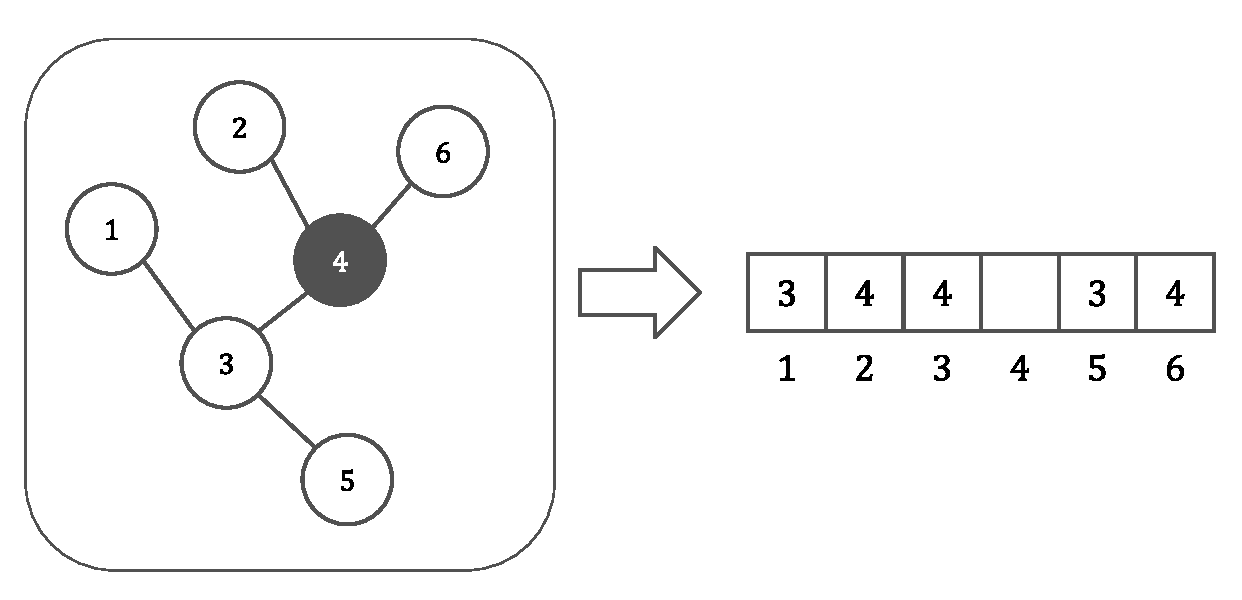
\includegraphics[scale=0.6]{files/graphs1.pdf}
  \caption{Exemplo de representação implícita de árvores, com vértice raiz realçado}
  \label{fig:graphs1}
\end{figure}

Esta \emph{eficiência} do teste de adjacência parece estar ligada ao fato da representação manter um número limitado de bits para cada vértice e utilizar apenas estes bits para o teste. Assim, podemos definir intuitivamente o conceito de representação implícita \footnote{Na literatura é usual definir como representação implícita apenas aquelas com $f(n) = n \log n$. A definição que apresentamos aqui é uma versão generalizada, formalizada em \cite{spinrad2003efficient}, que é mais apropriada para os problemas que trataremos a frente.} como a seguir:

Seja $C$ uma classe de grafos com $2^{\Theta(f(n))}$ elementos. Uma representação $R$ de um grafo $G \in C$, de $n$ vértices é dita implícita se:
\begin{enumerate}  
\item \emph{ela é assintoticamente ótima:} a representação requer apenas $O(f(n))$ bits no total;
\item \emph{ela distribui informação entre os vértices:} a representação local de cada vértice possui apenas $O(f(n)/n)$ bits;
\item \emph{o teste de adjacência é local:} para testar a adjacência entre dois vértices, apenas as informações locais a eles são necessárias.
\end{enumerate}

Um exemplo de classe que respeita essas propriedades são os \emph{grafos de intervalo}. Um grafo é dito de intervalo se cada um de seus vértices puder ser mapeado para um intervalo na reta real. Há aresta entre dois vértices se e somente se os respectivos intervalos possuem uma interseção não-vazia. Esta classe possui grande utilidade prática e pode ser definida uma representação implícita simples baseada na definição da classe. 

A representação consiste em enumerar as extremidades dos intervalos, na ordem em que aparecem na reta real, com inteiros no intervalo $[1..2n]$. Representa-se cada vértice do grafo com os dois inteiros correspondentes às extremidades de seu respectivo intervalo. Um exemplo pode ser visto na Figura~\ref{fig:graphs2}. Dois vértices serão considerados adjacentes se e somente se os intervalos representados pelos inteiros possuírem interseção não-vazia. Apenas $\Theta(\log n)$ bits são usados para representar cada vértice e $\Theta(n\log n)$ bits são usados para representar o grafo inteiro. Isto indica que há $2^{O(n \log n)}$ grafos de intervalo possíveis.

\begin{figure}[!htbp]
  \centering
  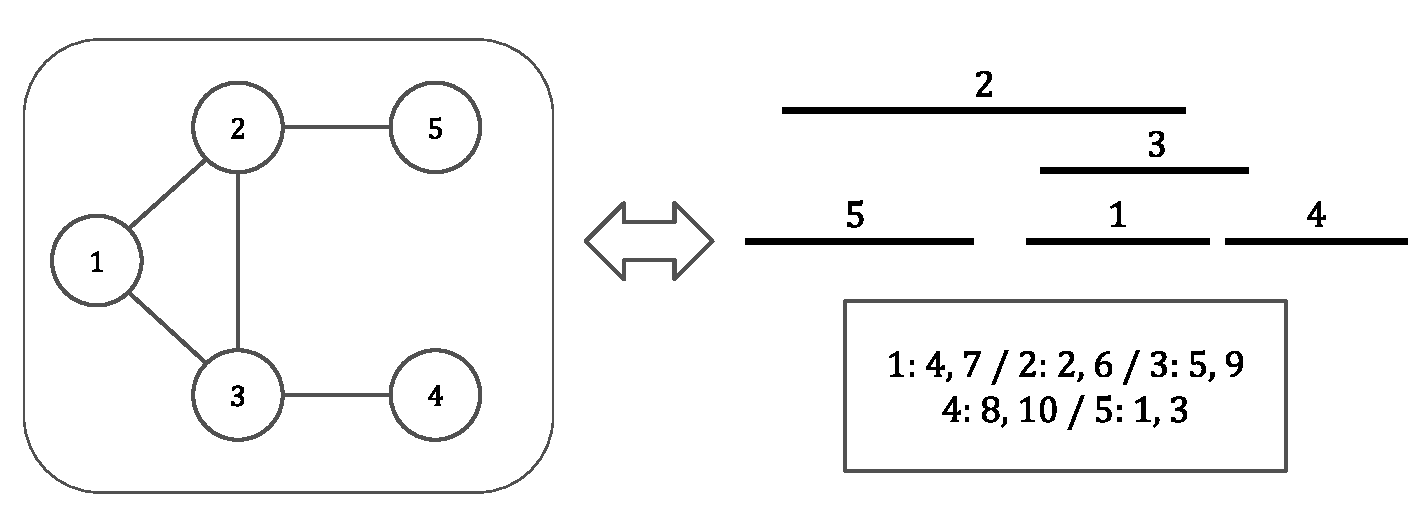
\includegraphics[scale=0.6]{files/graphs2.pdf}
  \caption{Exemplo de representação implícita de grafos de intervalo}
  \label{fig:graphs2}
\end{figure}


Para verificar o limite inferior no número de elementos na classe, considere grafos com $n$ vértices onde cada um dos $n/2$ primeiros vértices possuem uma aresta para um vértice distinto entre os $n/2$ últimos. Esta é uma subclasse dos grafos de intervalo. Por definição, ela possui $(n/2)!$ possíveis grafos com $n$ vértices. Como, $(n/2)!$ é $2^{\Theta(n \log n)}$, segue que há $2^{\Theta(n \log n)}$ grafos de intervalo e, portanto, a representação apresentada anteriormente é ótima.

Encontrar uma representação que respeite as propriedades necessárias pode não ser trivial. De fato, para muitas classes pode ser que não exista representação implícita. Por exemplo, considere a classe de grafos onde $m \leq n$. Usando uma lista de adjacência, é possível representar grafos nesta classe usando $O(n \log n)$ bits, o que indica que esta classe possui $2^{O(n\log n)}$ elementos. É impossível, entretanto, satisfazer as propriedades (2) e (3) simultaneamente, pois é possível transformar um grafo qualquer para um nesta classe introduzindo $n^2$ vértices de grau zero. Assim, se fosse houvesse uma representação implícita para este grafo, seria possível representar os $n$ vértices originais e suas adjacências usando apenas $O(n \log n)$ bits. Isto implicaria que é possível representar qualquer grafo usando $O(n \log n)$ bits, o que é absurdo.

A possibilidade de construir grafos em classes com $2^{\Theta(n\log n)}$ grafos a partir de grafos gerais apenas adicionando vértices pode posar como um desafio para definir propriedades gerais sobre essas classes. Por isso, utiliza-se mais frequentemente classes hereditárias na busca por classes com representações implícitas.

Uma classe é dita \emph{hereditária} se para todo grafo $G$ nesta classe, todo subgrafo induzido de $G$ também está na classe. A classe definida anteriormente (onde $m \leq n$) não é hereditária, pois a remoção de vértices de grafos naquela classe pode resultar em grafos fora dela. É possível provar que uma classe hereditária $C$ contém $2^{\Theta(n^2)}$ se e somente se ela contém todos os grafos bipartidos, todos os co-bipartidos ou todos os grafos \emph{split}.

É uma conjectura aberta se toda classe hereditária com $2^{O(n \log n)}$ grafos possui uma representação implícita. É conhecida como \emph{Conjectura da Representação Implícita} \cite{kannan1992implicat,spinrad2003efficient,chandoo2016implicit}. Importante notar que mesmo classes não-hereditárias podem possuir representação implícita (por exemplo, árvores).

%INCLUIR ALGO SOBRE REPRESENTAÇÕES PROBABILÍSTICAS

\subsection{Filtro de Bloom como representação implícita}\label{sec:graphs:repres}

Os resultados em \cite{pell2012scaling} e \cite{zhang2014these} suscitam a discussão sobre a viabilidade de representações probabilísticas para outras classes de grafos além dos de Bruijn.

Nesta seção, exploramos representações alternativas de grafos que utilizam estruturas de dados probabilísticas para permitir a estimativa das relações de adjacência entre os vértices. Deseja-se que, para determinadas classes de grafos, estas representações sejam pelo menos tão eficientes quanto as melhores representações conhecidas. Isto é, se uma classe $C$ possui $2^{\Theta(f(n))}$ grafos, o objetivo é derivar representações probabilísticas que requeiram $O(f(n))$ bits e permitam teste de adjacência com erro relativo constante $\epsilon$ e confiança $1 - \delta$.

Como exemplo, podemos estudar o uso direto de filtros de Bloom para representação do conjunto de arestas $E$ em grafos gerais. Como o objetivo é representar grafos gerais, o desejável é que seja possível construir o filtro com complexidade igual ou (preferencialmente) inferior a $\Theta(n^2)$. 

A ideia consiste em encontrar uma função \emph{hash} $h: E \to [1..m_B]$, que mapeia arestas do grafo em posições em um filtro de Bloom de $m_B$ bits.

De fato, filtros de Bloom permitem representar toda a adjacência do grafo utilizando 10 bits por aresta -- isto é, O(m) bits --, a fim de alcançar uma probabilidade de falsos positivos menor que 1\%. Esta representação mostra grande valor para representação de grafos esparsos, apesar de ser igualmente eficiente à matriz de adjacência ao requerer $\Theta(n^2)$ bits para representar o grafo no pior caso (ex.: grafos completos).

Esta representação possui uma característica importante: toda aresta do grafo é representada deterministicamente. Isto é, se a aresta existe no grafo original, com 100\% de probabilidade ela existirá na versão probabilística. Desta propriedade, segue que se um teste de adjacência na representação probabilística resultar em resposta negativa, é garantido que a aresta não exista no grafo original. Isto é, como característica do filtro de Bloom, não há falsos negativos. O contrário, entretanto, não é verdade. Em testes de adjacência entre vértices não-adjacentes, há probabilidade de falsos positivos. Isto significa, que para uma probabilidade de falsos positivos $p$, espera-se encontrar $p(\frac{n(n-1)}{2}-m)$ arestas na representação probabilística que não existem no grafo original.

É importante notar que, construída da forma apresentada, esta não seria uma representação implícita, mesmo se relaxarmos o requisito do teste de adjacência para permitir respostas probabilísticas. Isto se deve a esta representação não distribuir a informação entre os vértices. De fato, não há representação local nos vértices.

Uma variação que resolveria este problema seria manter um filtro de Bloom para cada vértice. Assim, para cada vértice $v$, teríamos um filtro de Bloom com $10 \times \text{d}(v)$ bits -- onde $\text{d}(v)$ é o grau do vértice -- de forma que a probabilidade de falsos positivos em cada um deles é exatamente igual e equivalente à versão anteriormente apresentada. Assim, para cada vértice, esta representação necessita de $O(\text{d}(v))$ bits que, no pior caso, é equivalente à matriz de adjacência ($O(n)$ bits), entretanto, permite representação de grafos esparsos com complexidade menor que a lista de adjacência, que requer $O(\text{d}(v) \log n)$ bits.

A Figura~\ref{fig:graph:bloom} compara os resultados empíricos para sucessivos testes em grafos aleatórios com $n = 1000$ e $m$ variando em todos os valores possíveis para um grafo com este tamanho. Ambas as variantes apresentadas nesta seção foram testadas. Note que para $m=0$, por característica da construção filtro de Bloom, não há arestas espúrias.

\begin{figure}[!htbp]
\centering
\scalebox{0.80}{\begin{tikzpicture}[
        declare function = {
            p(\n,\m) = 0.008193722*(\n*(\n-1)/2-\m);
        }
    ]
	\begin{axis}[
	    title=Filtro de Bloom único,
	    scaled ticks=false, 
        grid=both,
        ylabel={arestas espúrias},
    	xlabel=número de arestas ($m$),
        xmin=0, xmax=5000,
        ymin=0, ymax=50,
		legend columns=1, 
	    legend style={legend pos=outer north east,}
    ]

	\addplot[line width=1pt, mark=*,black,smooth, mark options={scale=0.75}] table[x=m,y=v1] {files/graph_bloom.txt};
	\addplot[smooth, mark options={scale=0.75}, line width=5pt,color={rgb:black,1;white,1},opacity=0.4] table[x=m,y=e] {files/graph_bloom.txt};
    %\addplot[dotted, line width=1pt, mark=none,black,smooth] table[x=k,y=max] {files/minhash_shakespeare.txt};
	%\legend{esperado,shakespeare, $\pm 1 \sigma$, min/max };


	\end{axis}
\end{tikzpicture} \begin{tikzpicture}[
        declare function = {
            p(\n,\m) = 0.008193*(\n*(\n-1)/2-\m);
        }
    ]
	\begin{axis}[
	    title=Um fitro de Bloom para cada vértice,
	    scaled ticks=false, 
        grid=both,
        xmin=0, xmax=5000,
        ymin=0, ymax=50,
		xlabel=número de arestas ($m$),
		yticklabel={\ },
		legend columns=1, 
	    %legend style={legend pos=outer north east,}
    ]

	\addplot[line width=1pt, mark=*,black,smooth, mark options={scale=0.75}] table[x=m,y=v2] {files/graph_bloom.txt};
	\addplot[smooth, mark options={scale=0.75}, line width=5pt,color={rgb:black,1;white,1},opacity=0.4] table[x=m,y=e] {files/graph_bloom.txt};
    %\addplot[dotted, line width=1pt, mark=none,black,smooth] table[x=k,y=max] {files/minhash_shakespeare2.txt};
	\legend{observado, esperado};

	\end{axis}
\end{tikzpicture}}
\caption{Arestas espúras em um grafo com $n=1000$.}
\label{fig:graph:bloom}
\end{figure}

\subsection{\emph{MinHash} como representação implícita}


\section{Conclusão}

\subsection{Futuros trabalhos}


\linespread{1}\selectfont
\bibliographystyle{alpha}
\bibliography{main}

\end{document}